\section{Langkah-Langkah Percobaan}
\subsection{Routing Statis IPv6}
\begin{enumerate}
	\item Mereset router ke konfigurasi awal.
	\item Melakukan enable IPv6 bila belum enabled, lalu restart router.
	\item Melakukan konfigurasi IP address pada ether1 sebagai jalur antar router. Untuk router pertama menggunakan address 2001:db8:1::1/64 dan router kedua menggunakan address 2001:db8:1::2/64.
	\item Melakukan konfigurasi IP address pada ether2 untuk router pertama dan ether4 untuk router kedua sebagai jalur antara router dengan laptop. Untuk router pertama menggunakan address 2001:db8:a::1/64 dan router kedua menggunakan address 2001:db8:b::1/64.
	\begin{figure}[H]
		\centering
		\begin{subfigure}[b]{0.4\linewidth}
			\centering
			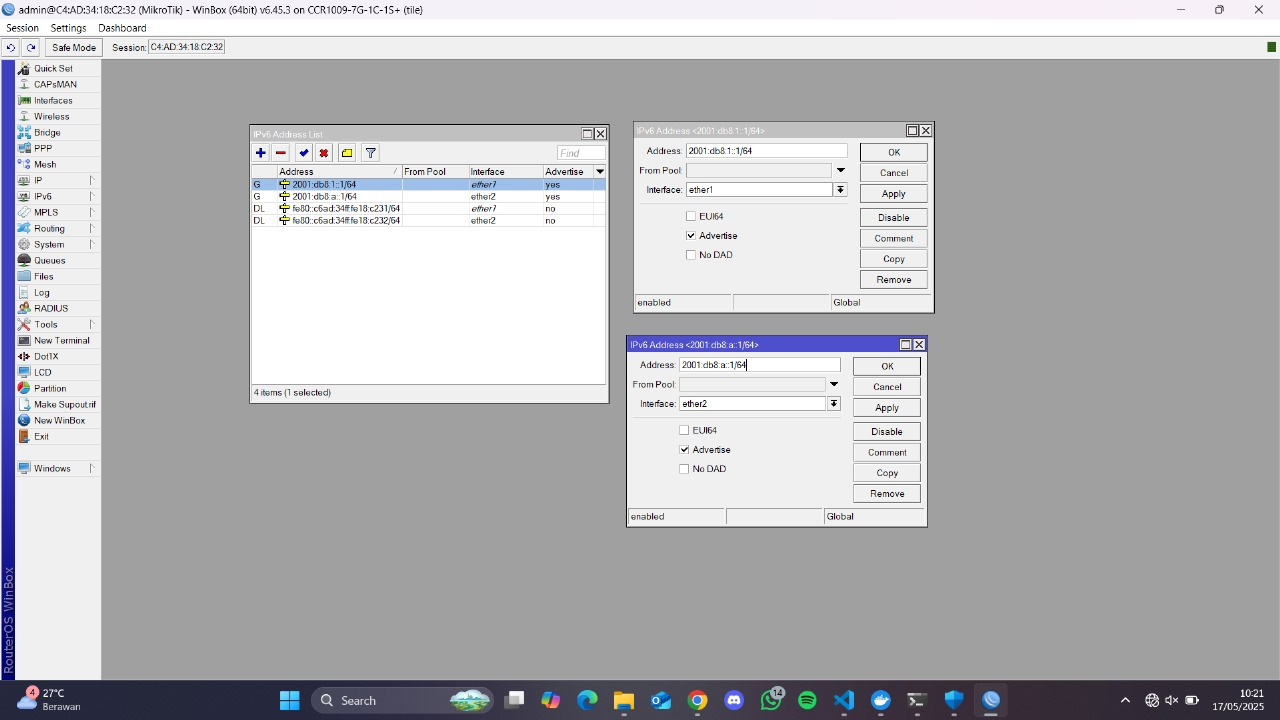
\includegraphics[width=\linewidth]{P2/img/router 1 laptop 1 (4).jpg}
			\caption{Konfigurasi ether1 dan ether2 router pertama\label{fig:konfigurasiR1}}
		\end{subfigure}
		\begin{subfigure}[b]{0.4\linewidth}
			\centering
			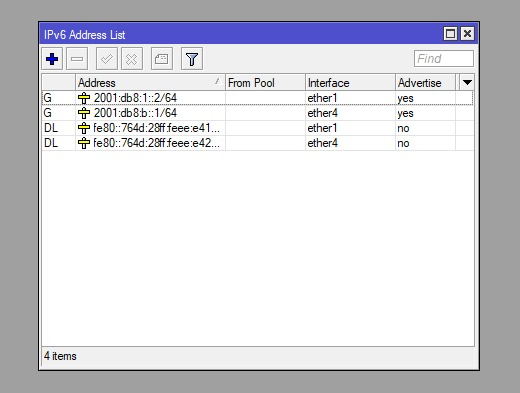
\includegraphics[width=\linewidth]{P2/img/router2 laptop2 (1).jpg}
			\caption{Konfigurasi ether1 dan ether4 router kedua\label{fig:konfigurasiR2}}
		\end{subfigure}
		\caption{Konfigurasi IP address pada router}
		\hspace{1cm}
	\end{figure}
	\item Melakukan konfigurasi routing statis pada router. Untuk router pertama ditambahkan rute dengan destination 2001:db8:b::/64 dan gateway 2001:db8:1::2. Untuk router kedua ditambagkan rute dengan destination 2001:db8:a::/64 dan gateway 2001:db8:1::1.
	\begin{figure}[H]
		\centering
		\begin{subfigure}[b]{0.4\linewidth}
			\centering
			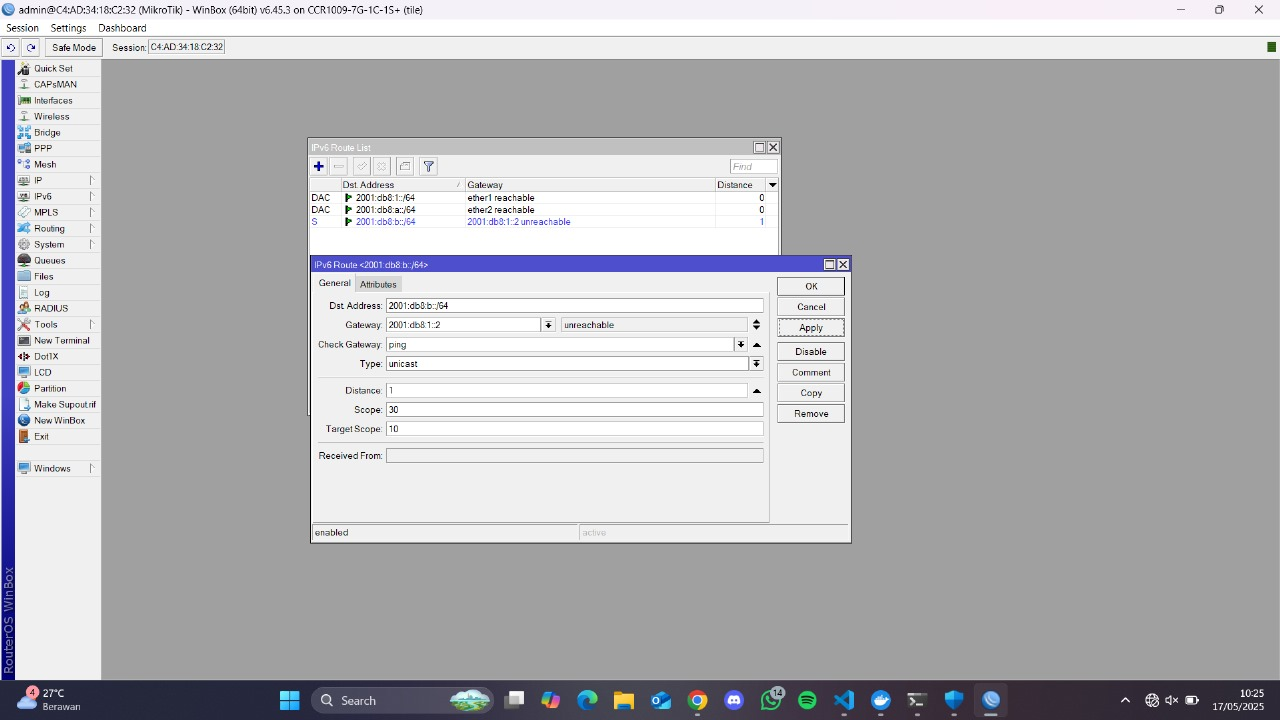
\includegraphics[width=\linewidth]{P2/img/router 1 laptop 1 (3).jpg}
			\caption{Konfigurasi routing statis router pertama\label{fig:konfigurasiR1}}
		\end{subfigure}
		\begin{subfigure}[b]{0.4\linewidth}
			\centering
			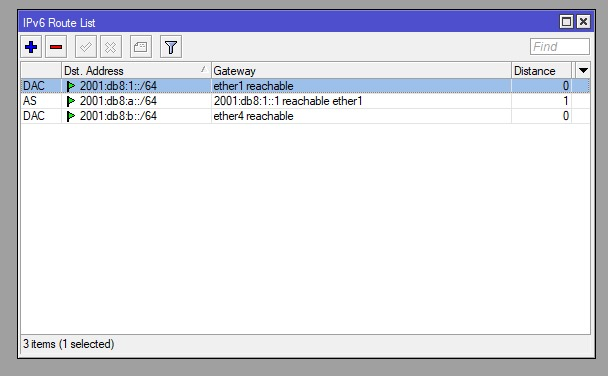
\includegraphics[width=\linewidth]{P2/img/router2 laptop2 (2).jpg}
			\caption{Konfigurasi routing statis router kedua\label{fig:konfigurasiR2}}
		\end{subfigure}
		\caption{Konfigurasi routing statis router}
		\hspace{1cm}
	\end{figure}
	\item Melakukan ping antar router. Pada router pertama menggunakan perintah ping 2001:db8:b::1. Pada router kedua menggunakan perintah 2001:db8:a::1.
	\item Melakukan konfigurasi IPv6 statis pada laptop. Untuk laptop pertama menggunakan konfigurasi address 2001:db8:a::100/64, gateway 2001:db8:a::1, dan DNS 2001:4860:4860::8888. Untuk laptop kedua menggunakan konfigurasi address 2001:db8:b::100/64, gateway 2001:db8:b::1, dan DNS 2001:4860:4860::8888.
	\begin{figure}[H]
		\centering
		\begin{subfigure}[b]{0.4\linewidth}
			\centering
			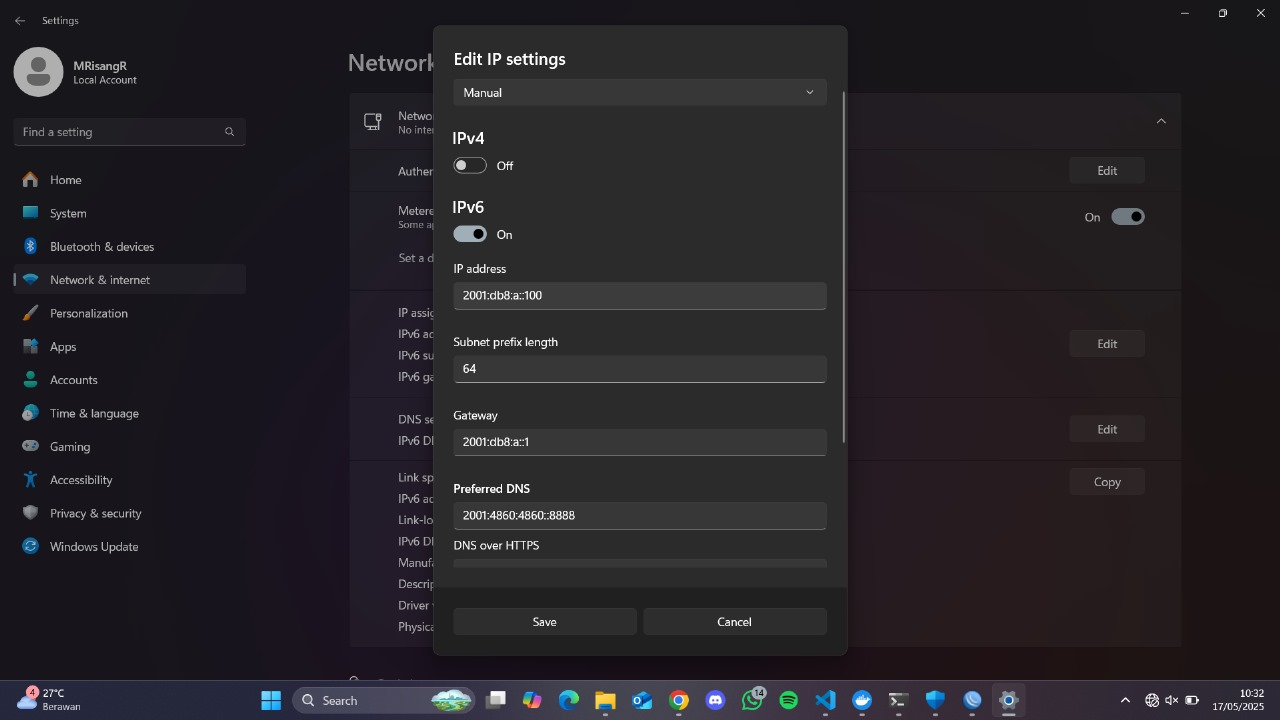
\includegraphics[width=\linewidth]{P2/img/router 1 laptop 1 (2).jpg}
			\caption{Konfigurasi IP address laptop pertama\label{fig:konfigurasiR1}}
		\end{subfigure}
		\begin{subfigure}[b]{0.4\linewidth}
			\centering
			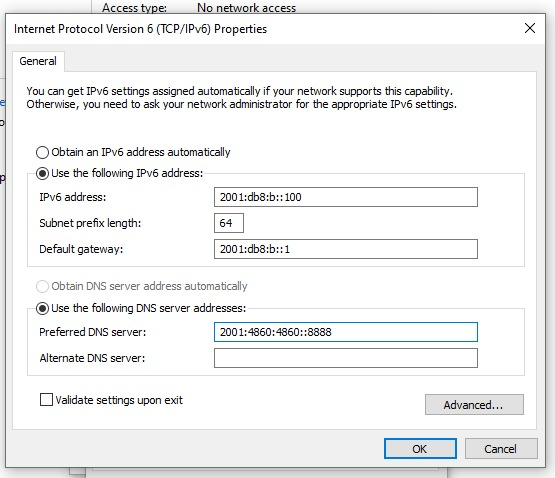
\includegraphics[width=\linewidth]{P2/img/router2 laptop2 (3).jpg}
			\caption{Konfigurasi IP address laptop kedua\label{fig:konfigurasiR2}}
		\end{subfigure}
		\caption{Konfigurasi IP address pada laptop}
		\hspace{1cm}
	\end{figure}
	\item Melakukan ping antar laptop. Pada laptop pertama menggunakan perintah ping 2001:db8:b::100. Pada router kedua menggunakan perintah ping 2001:db8:a::100.
	\begin{figure}[H]
		\centering
		\begin{subfigure}[b]{0.4\linewidth}
			\centering
			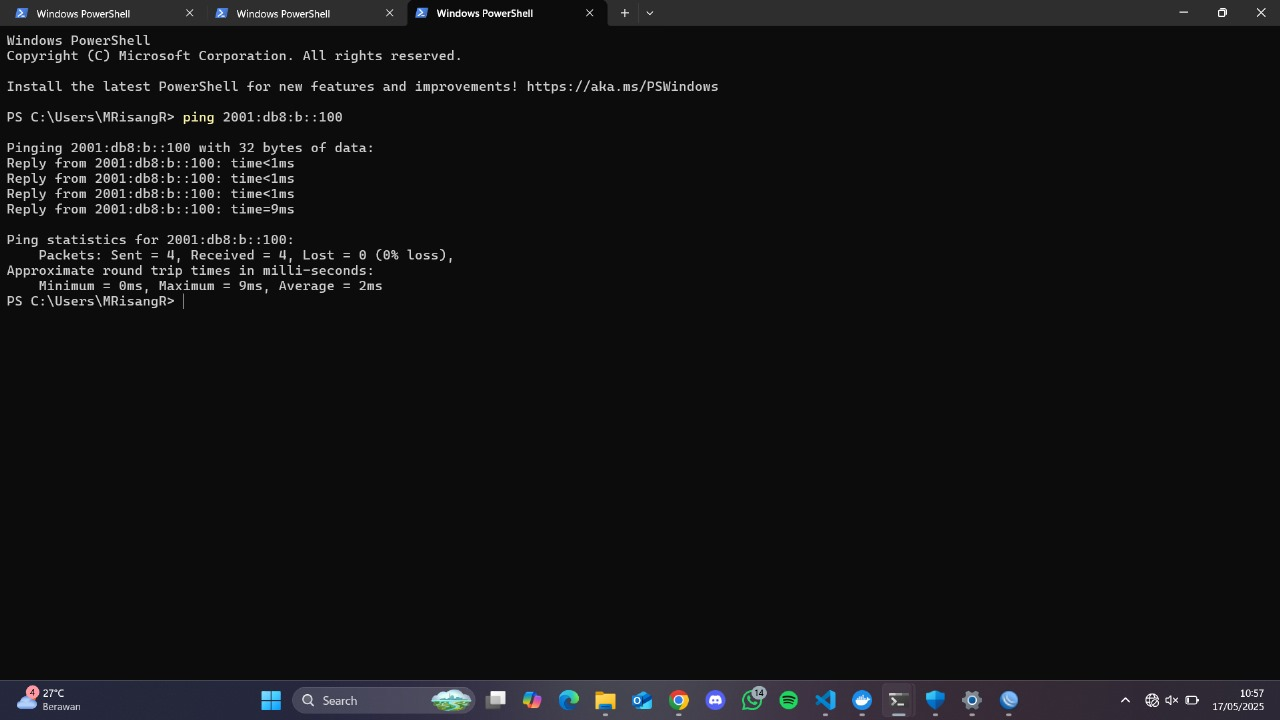
\includegraphics[width=\linewidth]{P2/img/router 1 laptop 1 (6).jpg}
			\caption{Ping laptop pertama (2001:db8:a::100) ke laptop kedua (2001:db8:b::100)\label{fig:konfigurasiR1}}
		\end{subfigure}
		\begin{subfigure}[b]{0.4\linewidth}
			\centering
			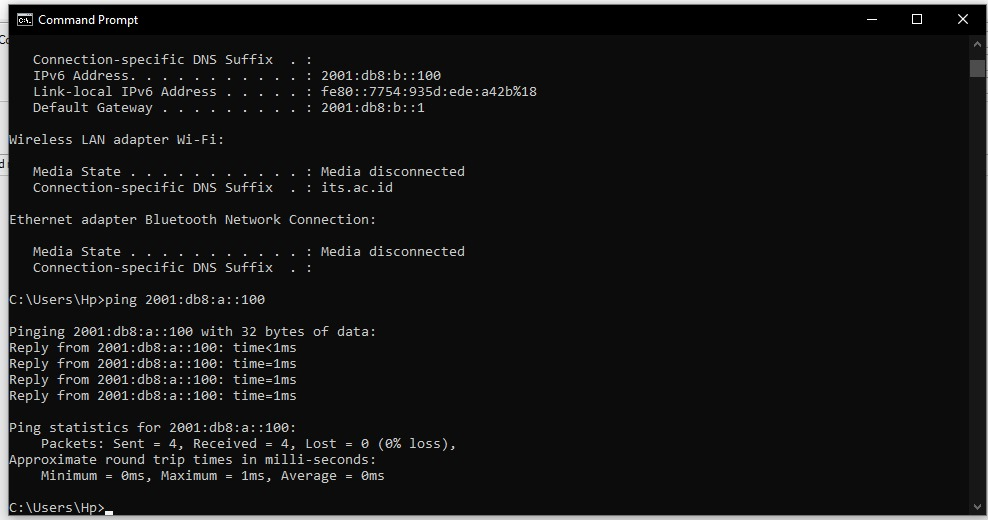
\includegraphics[width=\linewidth]{P2/img/router2 laptop2 (4).jpg}
			\caption{Ping laptop kedua (2001:db8:b::100) ke laptop pertama (2001:db8:a::100)\label{fig:konfigurasiR2}}
		\end{subfigure}
		\caption{Hasil ping antar laptop menggunakan routing statis}
		\hspace{1cm}
	\end{figure}
\end{enumerate}
\subsection{Routing Dinamis IPv4}
\begin{enumerate}
	\item Mereset router ke konfigurasi awal.
	\item Melakukan enable IPv6 bila belum enabled, lalu restart router.
	\item Melakukan konfigurasi IP address pada ether1 sebagai jalur antar router. Untuk router pertama menggunakan address 2001:db8:1::1/64 dan router kedua menggunakan address 2001:db8:1::2/64.
	\item Melakukan konfigurasi IP address pada ether2 untuk router pertama dan ether4 untuk router kedua sebagai jalur antara router dengan laptop. Untuk router pertama menggunakan address 2001:db8:a::1/64 dan router kedua menggunakan address 2001:db8:b::1/64.
	\begin{figure}[H]
		\centering
		\begin{subfigure}[b]{0.4\linewidth}
			\centering
			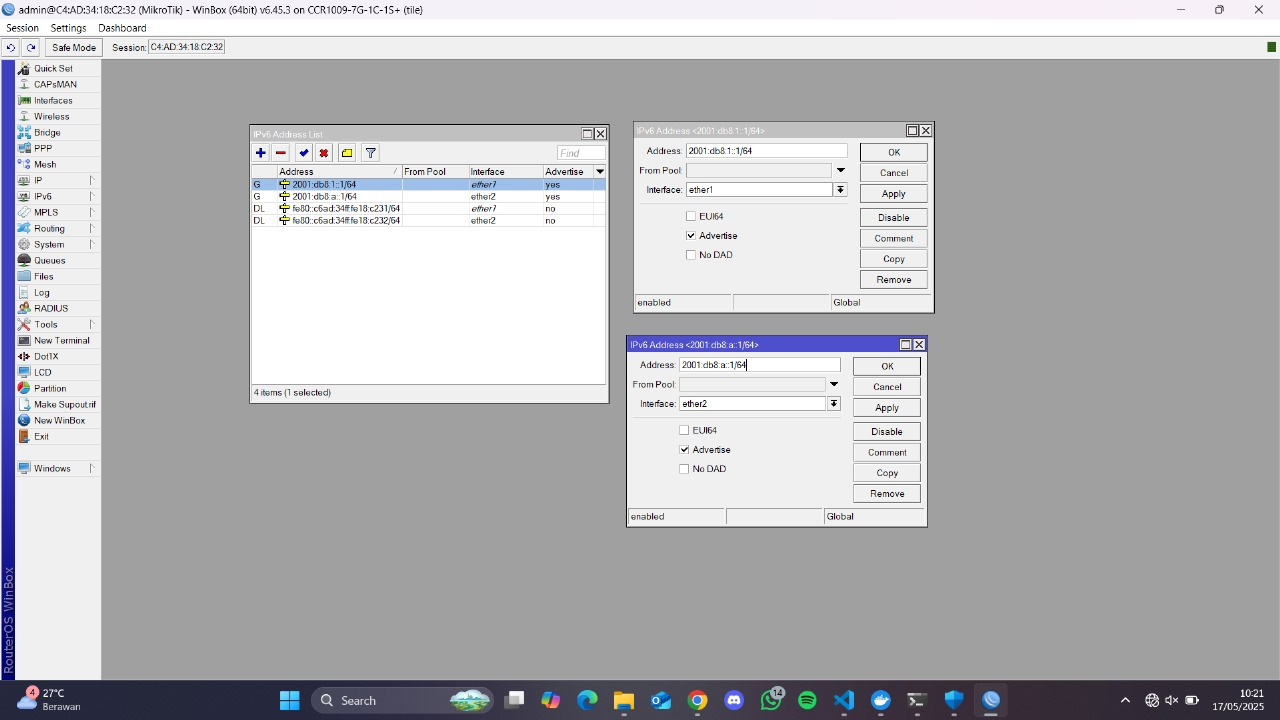
\includegraphics[width=\linewidth]{P2/img/router 1 laptop 1 (4).jpg}
			\caption{Konfigurasi ether1 dan ether2 router pertama\label{fig:konfigurasiR1}}
		\end{subfigure}
		\begin{subfigure}[b]{0.4\linewidth}
			\centering
			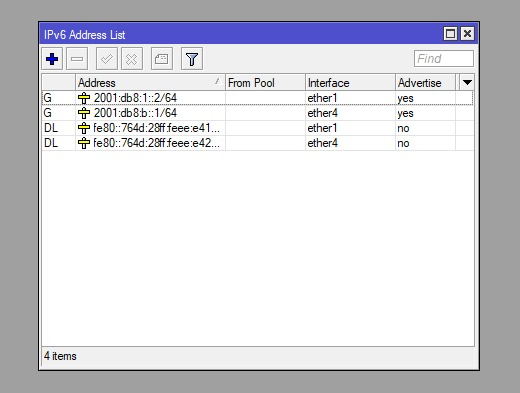
\includegraphics[width=\linewidth]{P2/img/router2 laptop2 (1).jpg}
			\caption{Konfigurasi ether1 dan ether4 router kedua\label{fig:konfigurasiR2}}
		\end{subfigure}
		\caption{Konfigurasi IP address pada router}
		\hspace{1cm}
	\end{figure}
	\item Melakukan routing dinamis pada router dengan membuat instance OSPF. Beri nama instance ospf-instance dan router ID 1.1.1.1 untuk router pertama dan 2.2.2.2 untuk router kedua.
	\begin{figure}[H]
		\centering
		\begin{subfigure}[b]{0.4\linewidth}
			\centering
			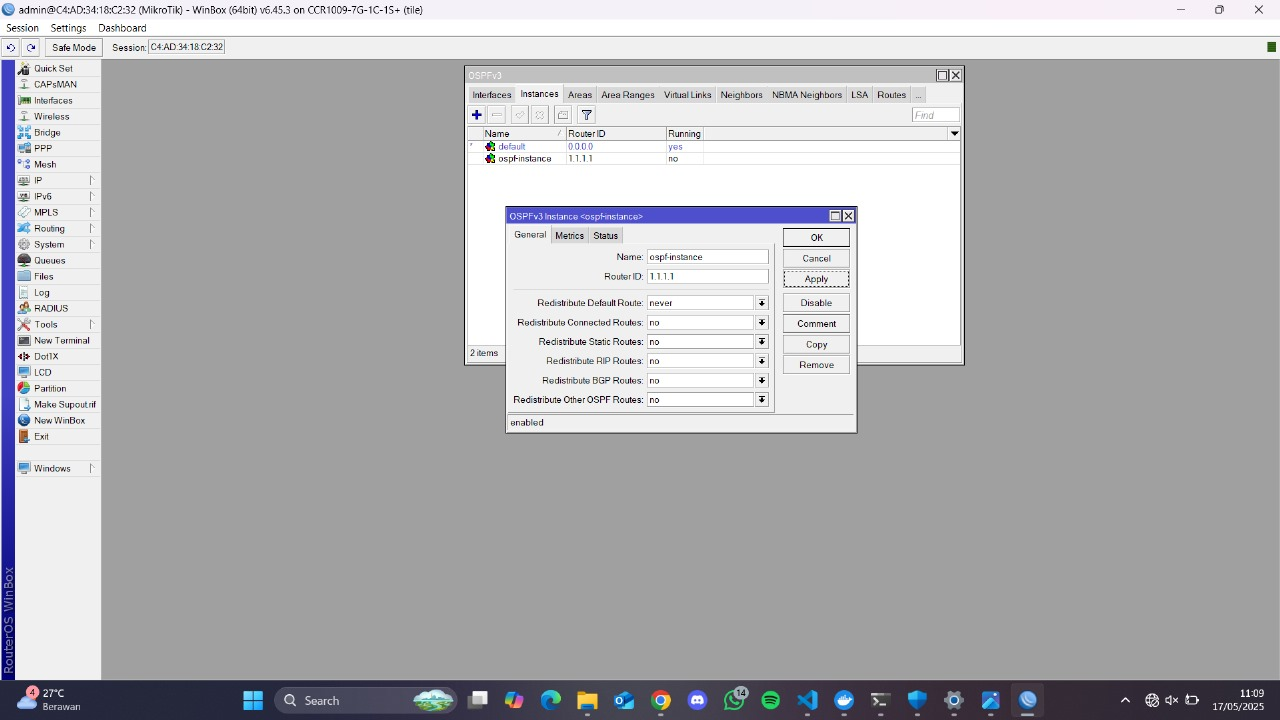
\includegraphics[width=\linewidth]{P2/img/router 1 laptop 1 (7).jpg}
			\caption{Konfigurasi OSPF instance pada router pertama\label{fig:konfigurasiR1}}
		\end{subfigure}
		\begin{subfigure}[b]{0.4\linewidth}
			\centering
			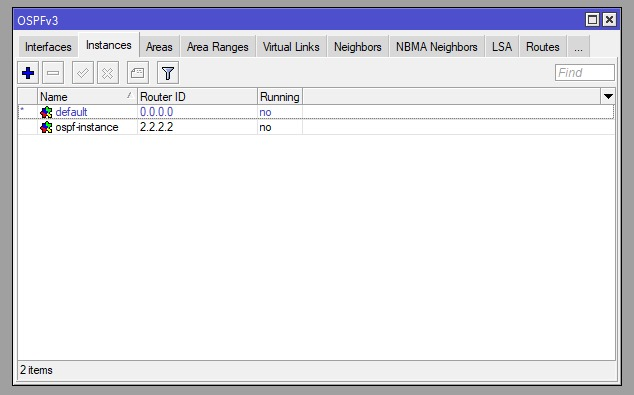
\includegraphics[width=\linewidth]{P2/img/router2 laptop2 (5).jpg}
			\caption{Konfigurasi OSPF instance pada router kedua\label{fig:konfigurasiR2}}
		\end{subfigure}
		\caption{Konfigurasi OSPF instance}
		\hspace{1cm}
	\end{figure}
	\item Menambahkan area baru pada OSPF, dengan nama area1, instance ospf-instance, dan area ID 0.0.0.0.
	\begin{figure}[H]
		\centering
			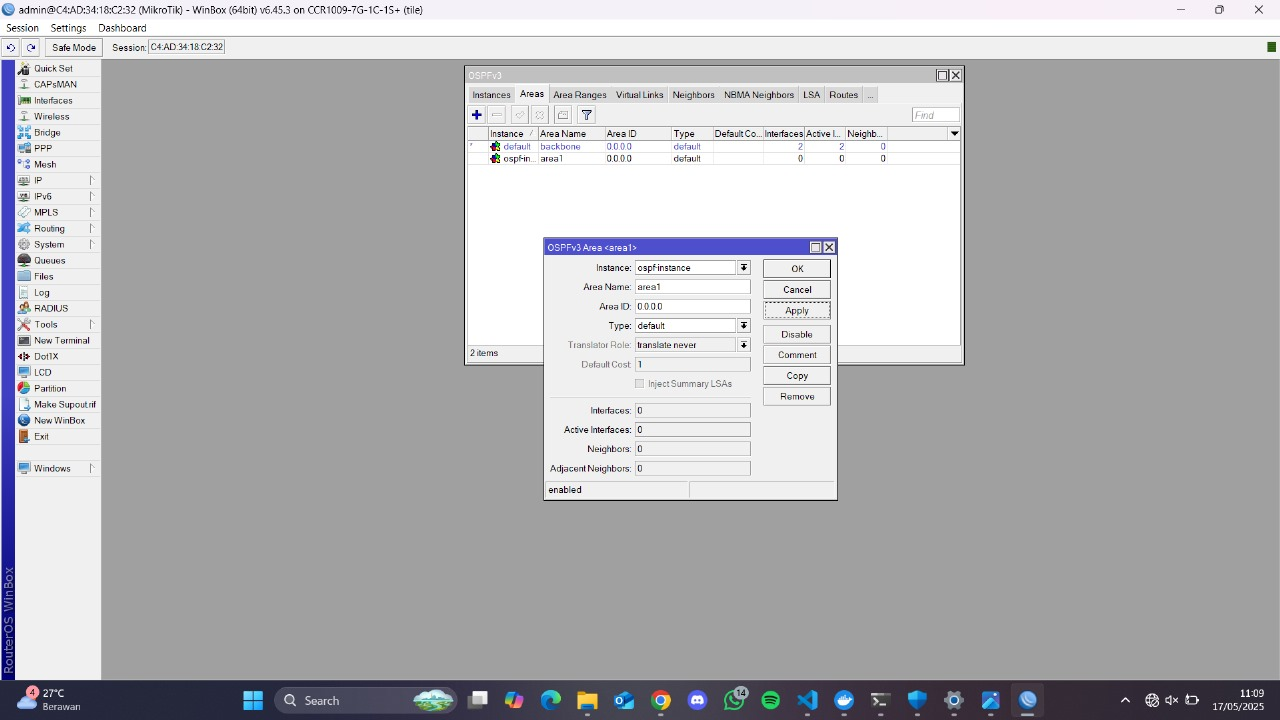
\includegraphics[width=\linewidth]{P2/img/router 1 laptop 1 (13).jpg}
		\caption{Konfigurasi area OSPF}
		\hspace{1cm}
	\end{figure}
	\item Menambahkan interface baru untuk setiap interface router (pada router pertama ehter1 dan ether2, pada router kedua ether1 dan ether4) dengan konfigurasi area area1.
	\begin{figure}[H]
			\centering
			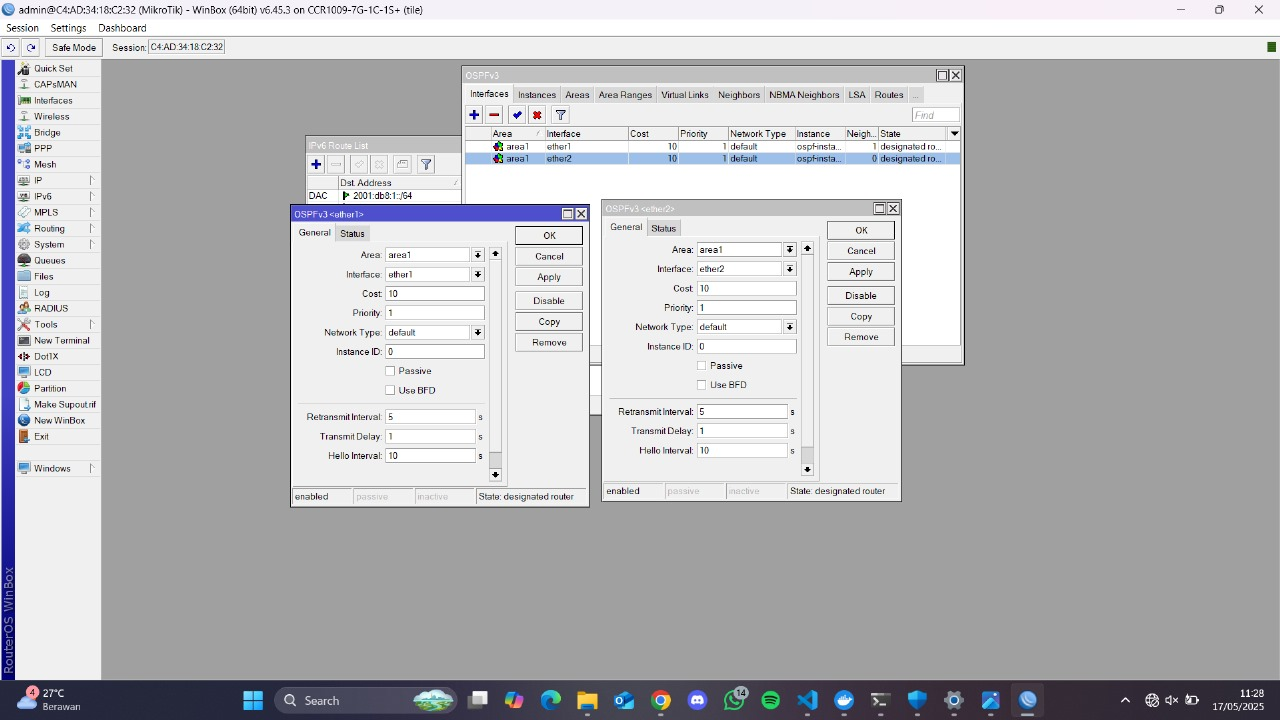
\includegraphics[width=\linewidth]{P2/img/router 1 laptop 1 (10).jpg}
		\caption{Konfigurasi interface OSPF}
		\hspace{1cm}
	\end{figure}
	\item Memeriksa OSPF neighbor dan routing. Pada router pertama, harus muncul neighbor dengan router ID 2.2.2.2 (router kedua). Pada router kedua harus muncul neighbor dengan router ID 1.1.1.1 (router pertama).
	\begin{figure}[H]
		\centering
		\begin{subfigure}[b]{0.4\linewidth}
			\centering
			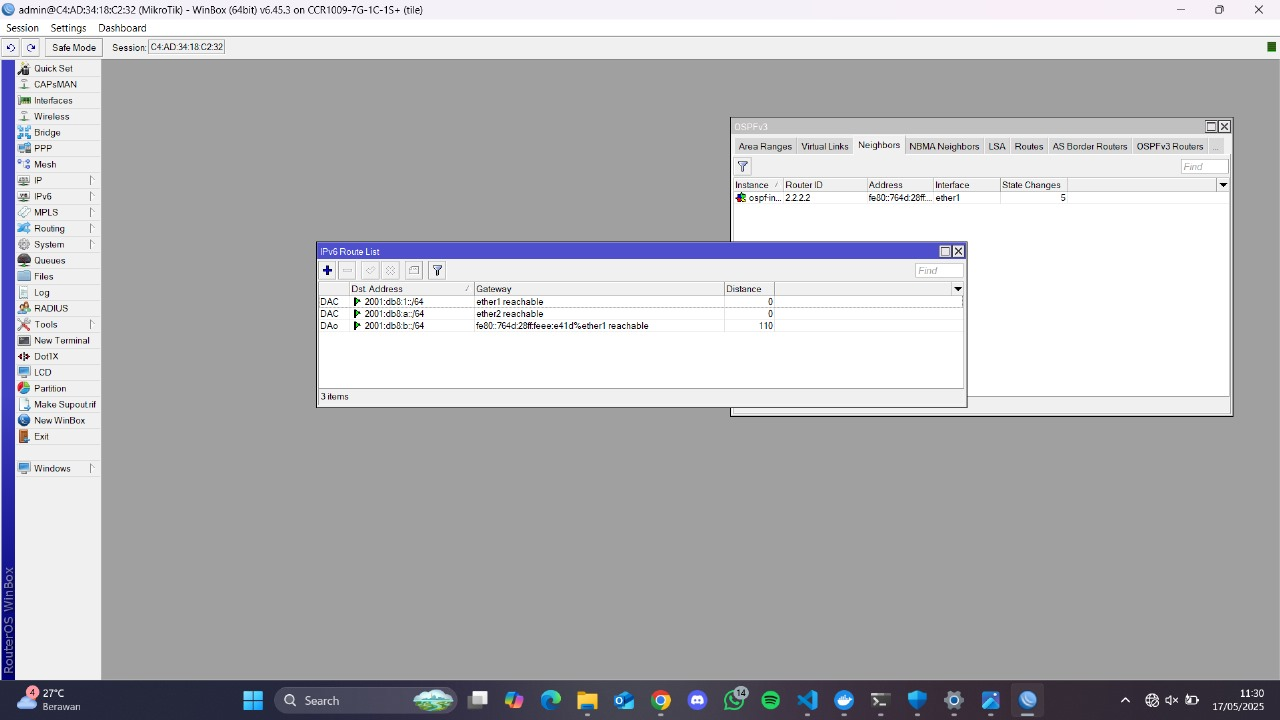
\includegraphics[width=\linewidth]{P2/img/router 1 laptop 1 (12).jpg}
			\caption{OSPF neighbor dan route list router pertama\label{fig:konfigurasiR1}}
		\end{subfigure}
		\begin{subfigure}[b]{0.4\linewidth}
			\centering
			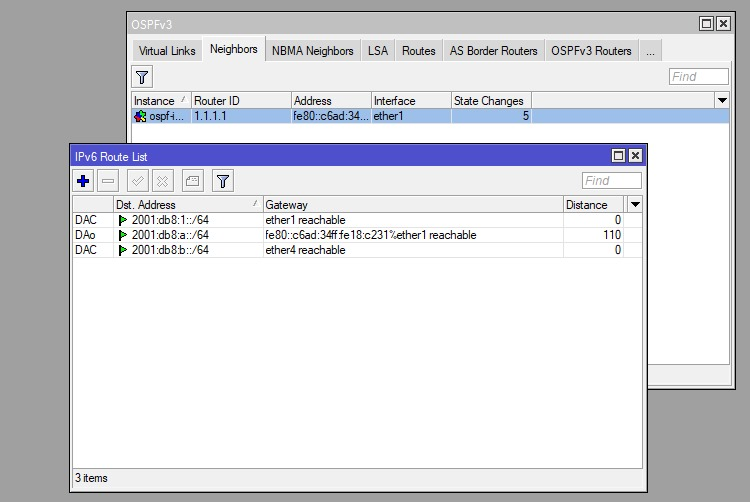
\includegraphics[width=\linewidth]{P2/img/router2 laptop2 (9).jpg}
			\caption{OSPF neighbor dan route list router kedua\label{fig:konfigurasiR2}}
		\end{subfigure}
		\caption{Pemeriksaan OSPF neighbor dan route list}
		\hspace{1cm}
	\end{figure}
	\item Melakukan ping antar router. Pada router pertama menggunakan perintah ping 2001:db8:b::1. Pada router kedua menggunakan perintah 2001:db8:a::1.
	\item Melakukan konfigurasi IPv6 statis pada laptop. Untuk laptop pertama menggunakan konfigurasi address 2001:db8:a::100/64, gateway 2001:db8:a::1, dan DNS 2001:4860:4860::8888. Untuk laptop kedua menggunakan konfigurasi address 2001:db8:b::100/64, gateway 2001:db8:b::1, dan DNS 2001:4860:4860::8888.
	\begin{figure}[H]
		\centering
		\begin{subfigure}[b]{0.4\linewidth}
			\centering
			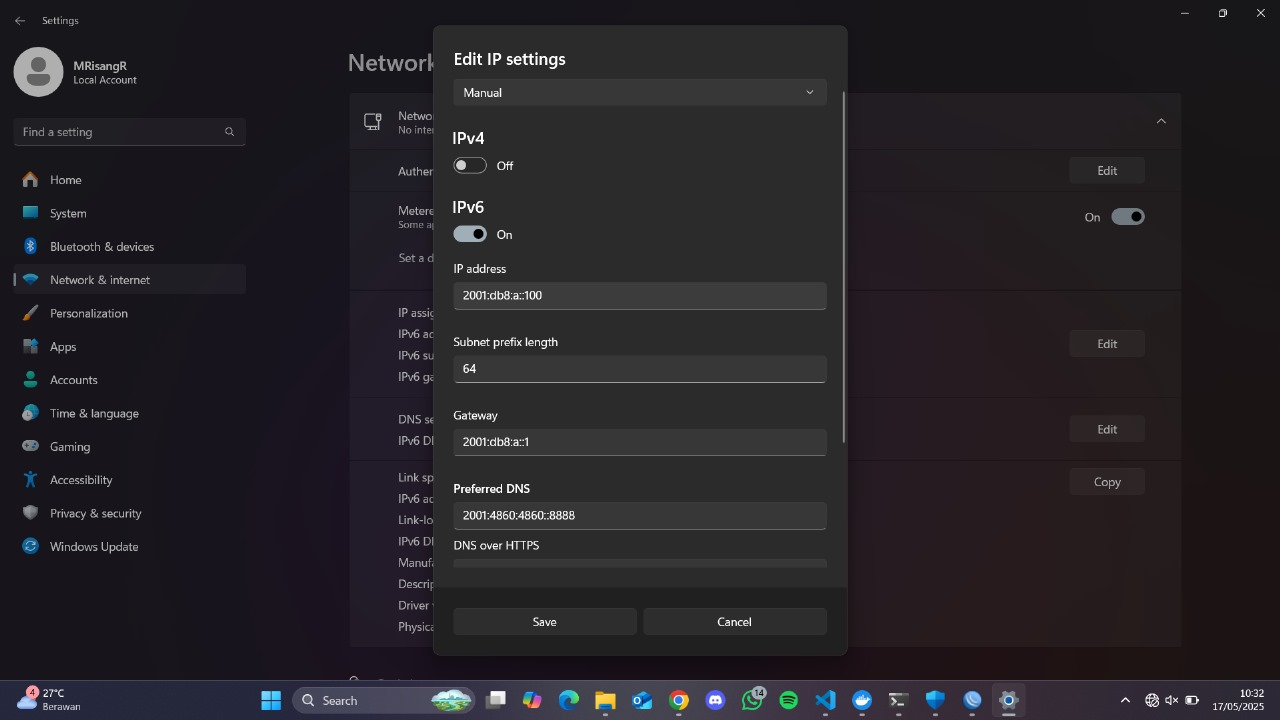
\includegraphics[width=\linewidth]{P2/img/router 1 laptop 1 (2).jpg}
			\caption{Konfigurasi IP address laptop pertama\label{fig:konfigurasiR1}}
		\end{subfigure}
		\begin{subfigure}[b]{0.4\linewidth}
			\centering
			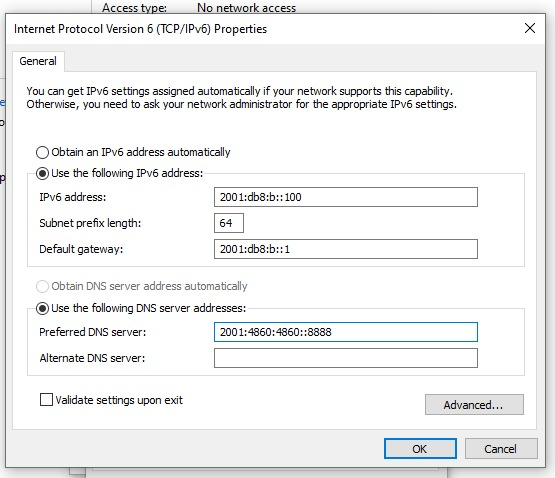
\includegraphics[width=\linewidth]{P2/img/router2 laptop2 (3).jpg}
			\caption{Konfigurasi IP address laptop kedua\label{fig:konfigurasiR2}}
		\end{subfigure}
		\caption{Konfigurasi IP address pada laptop}
		\hspace{1cm}
	\end{figure}
	\item Melakukan ping antar laptop. Pada laptop pertama menggunakan perintah ping 2001:db8:b::100. Pada router kedua menggunakan perintah ping 2001:db8:a::100.
	\begin{figure}[H]
		\centering
		\begin{subfigure}[b]{0.4\linewidth}
			\centering
			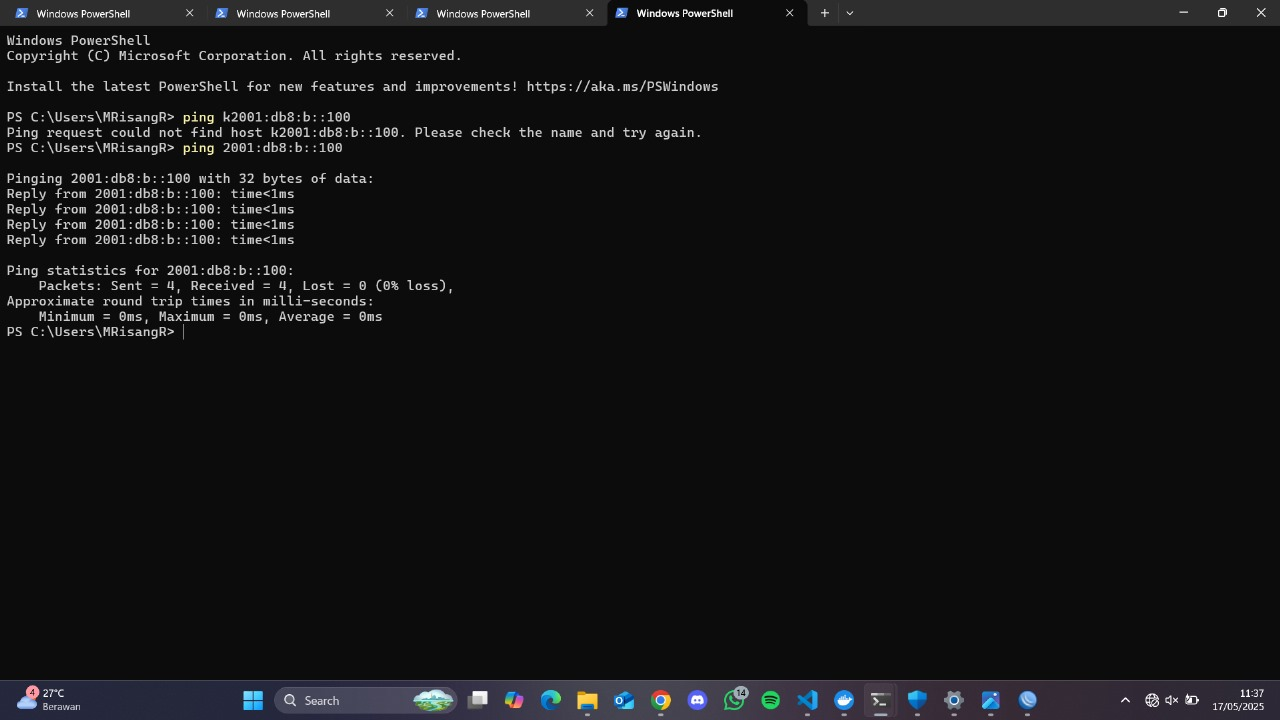
\includegraphics[width=\linewidth]{P2/img/router 1 laptop 1 (8).jpg}
			\caption{Ping laptop pertama (2001:db8:a::100) ke laptop kedua (2001:db8:b::100)\label{fig:konfigurasiR1}}
		\end{subfigure}
		\begin{subfigure}[b]{0.4\linewidth}
			\centering
			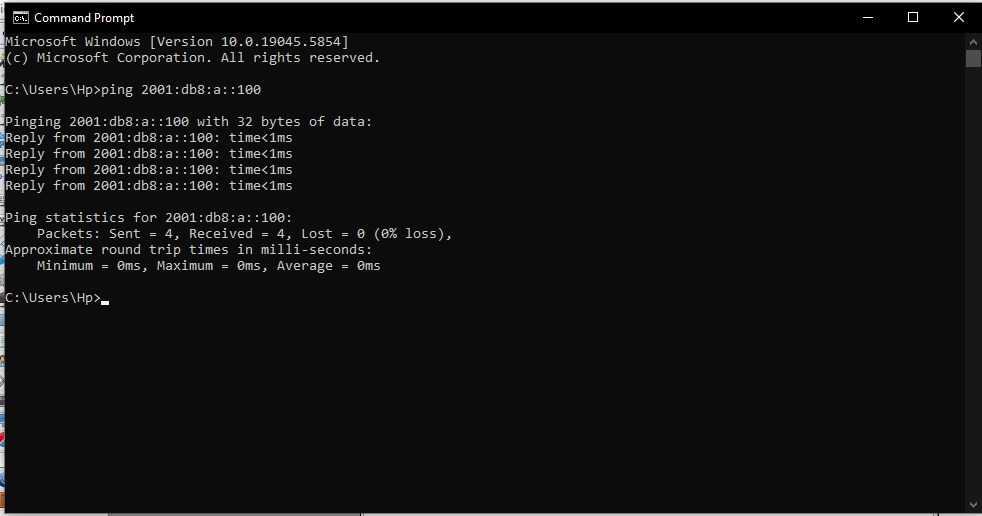
\includegraphics[width=\linewidth]{P2/img/router2 laptop2 (7).jpg}
			\caption{Ping laptop kedua (2001:db8:b::100) ke laptop pertama (2001:db8:a::100)\label{fig:konfigurasiR2}}
		\end{subfigure}
		\caption{Hasil ping antar laptop menggunakan routing dinamis}
		\hspace{1cm}
	\end{figure}
	
\end{enumerate}

\section{Analisis Hasil Percobaan}
\indent Pada praktikum ini, dilakukan 2 percobaan yaitu routing statis IPv6 dan routing dinamis IPv6. Percobaan pertama yang dilakukan adalah routing statis menggunakan IPv6. Routing statis memungkinkan router dan end device (seperti komputer dan laptop) untuk berkomunikasi melalui alamat IP yang telah ditetapkan/diatur secara manual dan tidak akan berubah sama sekali (statis) selama konfigurasinya tidak diubah atau router direset ke pengaturan awal. Bila konfigurasi routing benar, maka end device yang terhubung dalam jaringan akan mampu melakukan ping ke satu sama lain. Pada percobaan ini, dilakukan konfigurasi routing statis IPv6 menggunakan 2 router dan 2 laptop. Routing statis dilakukan dengan memberikan alamat IPv6 secara manual ke masing-masing router dan laptop, lalu mengatur gateway secara manual pula pada routing router dan laptop. Hasil akhir yang didapatkan pada percobaan ini adalah laptop pertama berhasil melakukan ping ke laptop kedua dan laptop kedua juga berhasil melakukan ping ke laptop pertama. Maka dari itu, dapat disimpulkan bahwa percobaan pertama berhasil dan hasil percobaannya sesuai dengan teori.
\begin{figure}[H]
	\centering
	\begin{subfigure}[b]{0.4\linewidth}
		\centering
		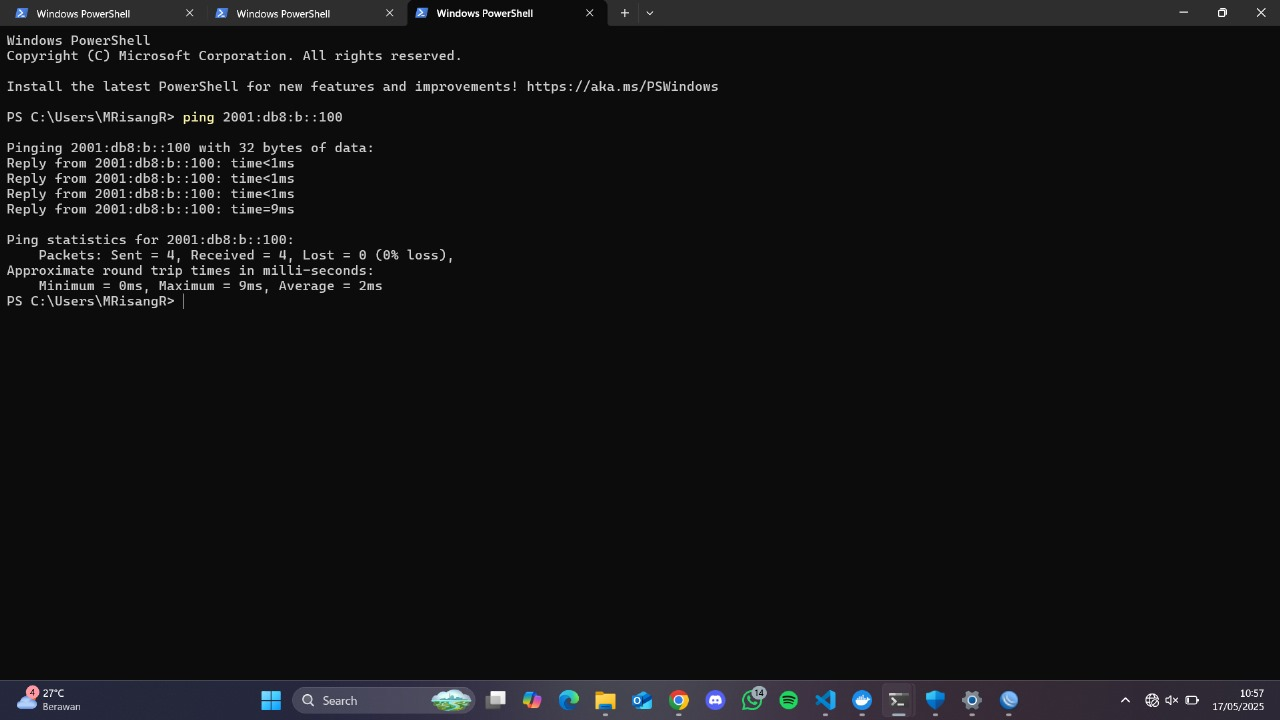
\includegraphics[width=\linewidth]{P2/img/router 1 laptop 1 (6).jpg}
		\caption{Ping laptop pertama (2001:db8:a::100) ke laptop kedua (2001:db8:b::100)\label{fig:konfigurasiR1}}
	\end{subfigure}
	\begin{subfigure}[b]{0.4\linewidth}
		\centering
		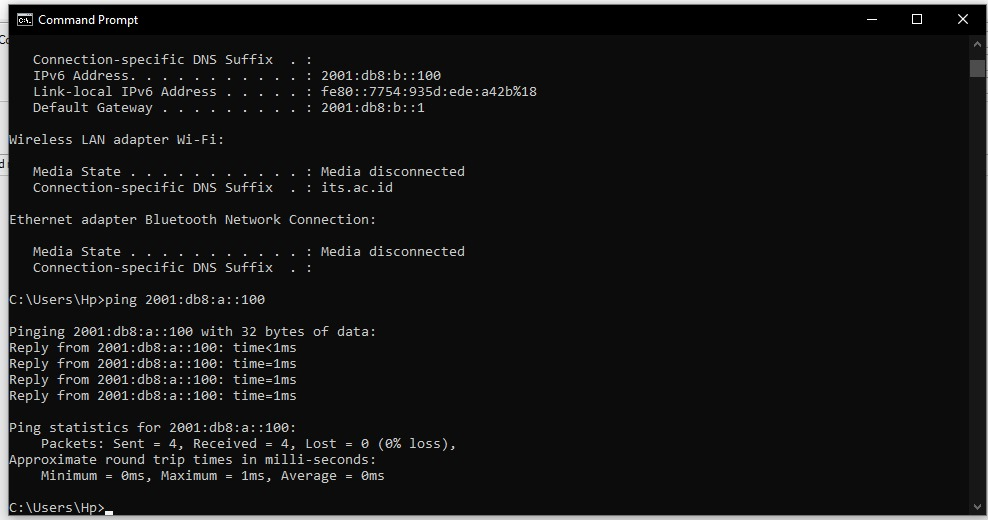
\includegraphics[width=\linewidth]{P2/img/router2 laptop2 (4).jpg}
		\caption{Ping laptop kedua (2001:db8:b::100) ke laptop pertama (2001:db8:a::100)\label{fig:konfigurasiR2}}
	\end{subfigure}
	\caption{Hasil ping antar laptop menggunakan routing statis}
	\hspace{1cm}
\end{figure}

Percobaan kedua yang dilakukan adalah routing dinamis menggunakan IPv6. Routing dinamis memungkinkan router dan end device untuk berkomunikasi melalui alamat IP yang digenerate secara otomatis tanpa harus memberikan alamat IP secara manual kepada masing-masing device, alamat IP yang digunakan oleh masing-masing router dan device pun akan berubah-ubah pada bagian host ID-nya (untuk alamat IPv6 dengan prefix /64, maka yang berubah adalah 64-bit atau 16-hex terakhir alamat). Bila konfigurasi berhasil, maka end device yang terhubung dalam jaringan akan mampu melakukan ping ke satu sama lain. Pada percobaan ini, dilakukan routing dinamis IPv6 menggunakan OSPFv3 dengan 2 router dan 2 laptop. Routing dinamis menggunakan OSPFv3 dilakukan untuk komunikasi antar router, sedangkan pada laptop tetap diberikan alamat IPv6 secara manual. Hasil akhir yang didapatkan pada percobaan ini adalah kedua router dapat berkomunikasi menggunakan routing dinamis dengan OSPFv3, yang dibuktikan dengan keberhasilan pengiriman ping antara laptop pertama dan laptop kedua. Maka dari itu, dapat disimpulkan bahwa percobaan kedua berhasil dan hasil percobaannya sesuai dengan teori.
\begin{figure}[H]
	\centering
	\begin{subfigure}[b]{0.4\linewidth}
		\centering
		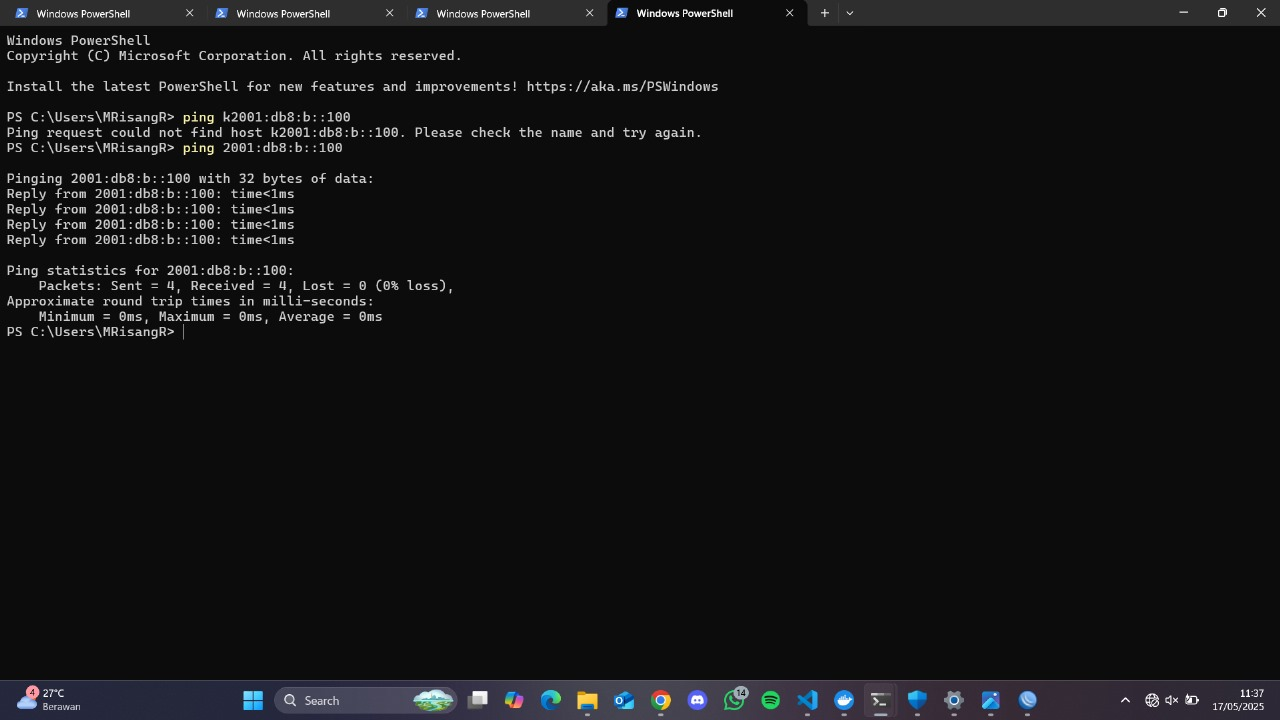
\includegraphics[width=\linewidth]{P2/img/router 1 laptop 1 (8).jpg}
		\caption{Ping laptop pertama (2001:db8:a::100) ke laptop kedua (2001:db8:b::100)\label{fig:konfigurasiR1}}
	\end{subfigure}
	\begin{subfigure}[b]{0.4\linewidth}
		\centering
		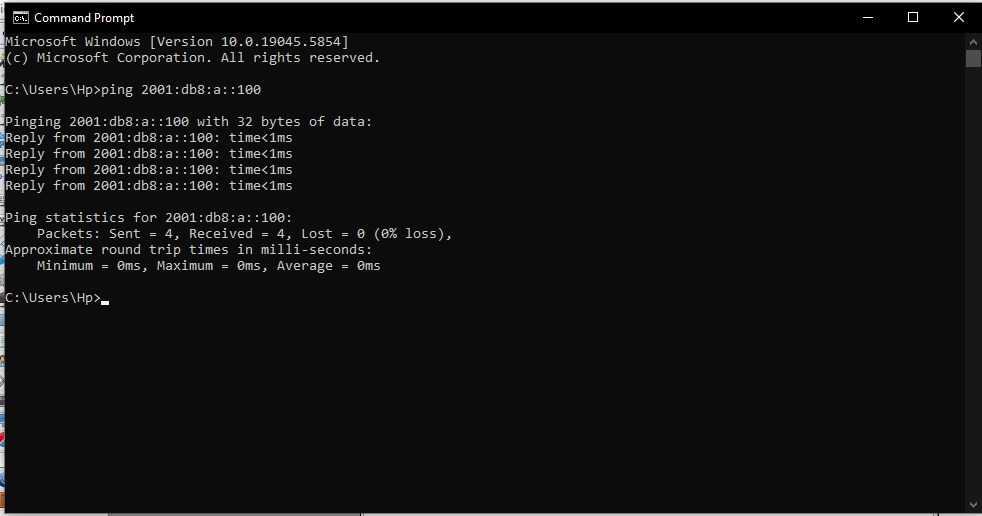
\includegraphics[width=\linewidth]{P2/img/router2 laptop2 (7).jpg}
		\caption{Ping laptop kedua (2001:db8:b::100) ke laptop pertama (2001:db8:a::100)\label{fig:konfigurasiR2}}
	\end{subfigure}
	\caption{Hasil ping antar laptop menggunakan routing dinamis}
	\hspace{1cm}
\end{figure}

\section{Hasil Tugas Modul}
Berikut merupakan hasil simulasi dari percobaan routing statis dan dinamis IPv6 menggunakan Cisco Packet Tracer:\\
Topologi jaringan:
\begin{figure}[H]
	\centering
	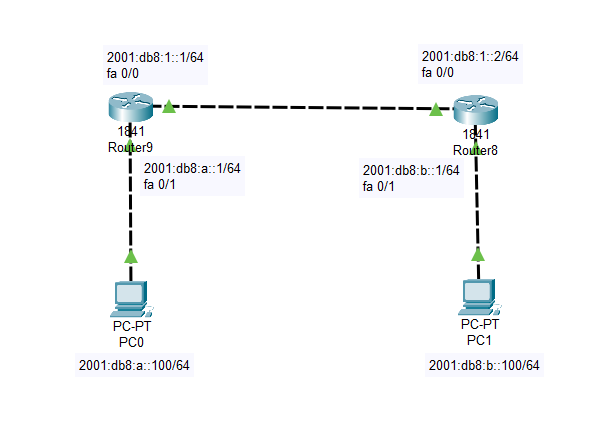
\includegraphics{P2/img/tumod (6).png}
	\caption{Topologi jaringan \label{fig:topologi}}
\end{figure}

Routing statis dan hasilnya:
\begin{figure}[H]
	\begin{subfigure}[b]{0.4\linewidth}
		\centering
		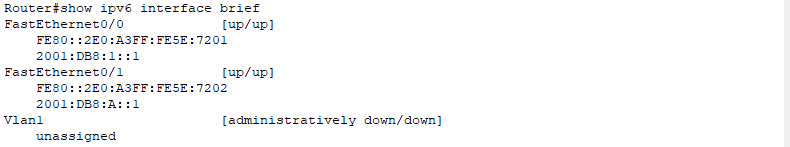
\includegraphics[width=\linewidth]{P2/img/tumod (9).png}
		\caption{Kofigurasi IPv6 router 1\label{fig:konfigurasiR1}}
	\end{subfigure}
	\begin{subfigure}[b]{0.4\linewidth}
		\centering
		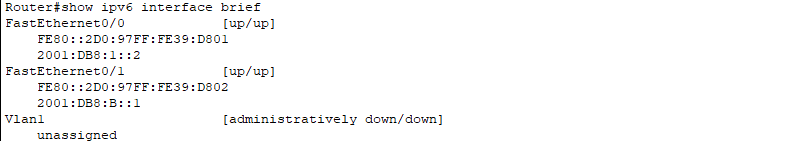
\includegraphics[width=\linewidth]{P2/img/tumod (11).png}
		\caption{Konfigurasi IPv6 router 2\label{fig:konfigurasiR2}}
	\end{subfigure}
	\hspace{1cm}
	\begin{subfigure}[b]{0.4\linewidth}
		\centering
		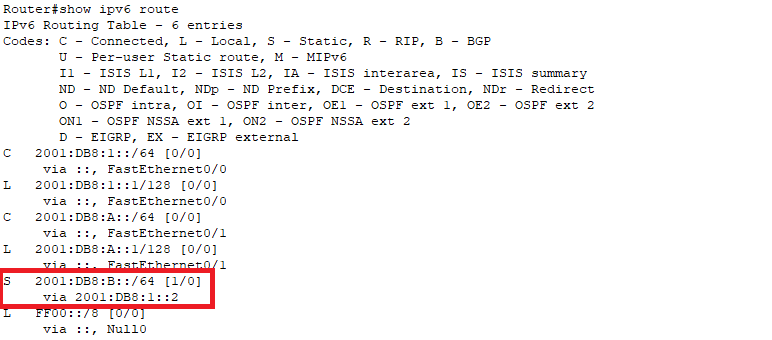
\includegraphics[width=\linewidth]{P2/img/tumod (10).png}
		\caption{Routing statis IPv6 router 1\label{fig:routingR1}}
	\end{subfigure}
	\begin{subfigure}[b]{0.4\linewidth}
		\centering
		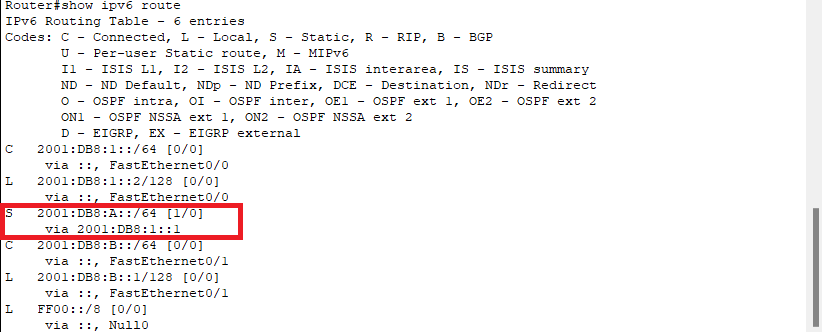
\includegraphics[width=\linewidth]{P2/img/tumod (1).png}
		\caption{Routing statis IPv6 router 2\label{fig:routingR2}}
	\end{subfigure}
	\hspace{1cm}
	\begin{subfigure}[b]{0.55\linewidth}
		\centering
		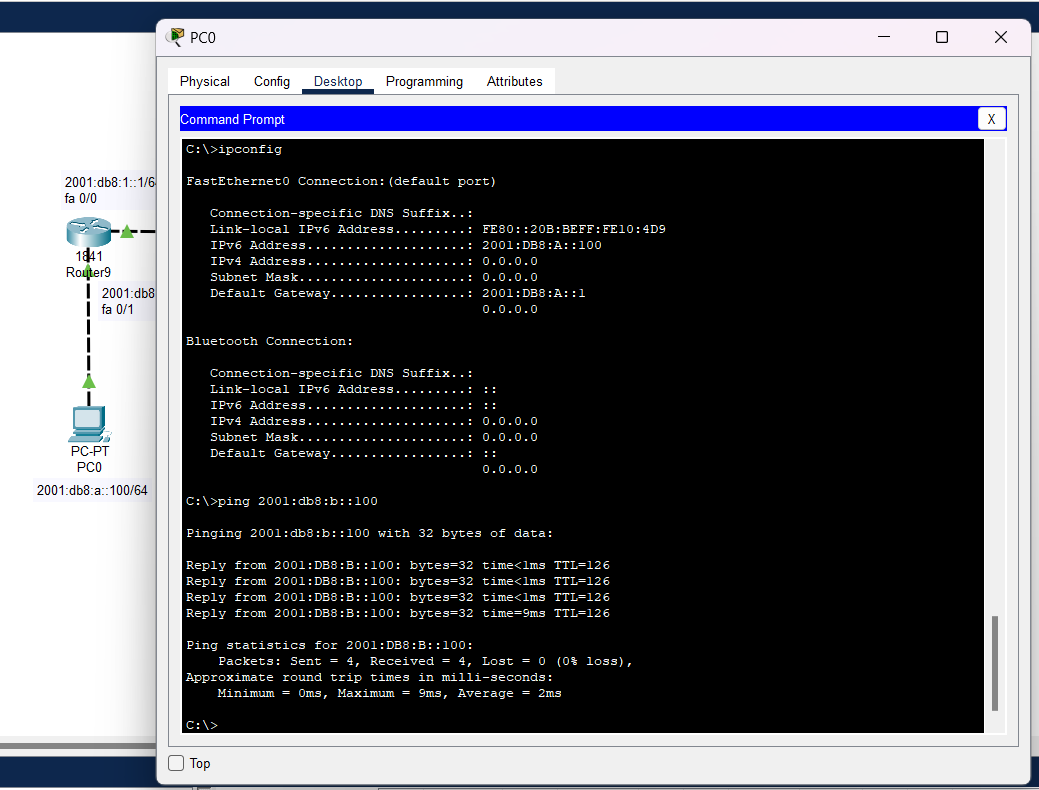
\includegraphics[width=\linewidth]{P2/img/tumod (7).png}
		\caption{Ping PC 1 ke PC 2\label{fig:pingPC1}}
	\end{subfigure}
	\begin{subfigure}[b]{0.5\linewidth}
		\centering
		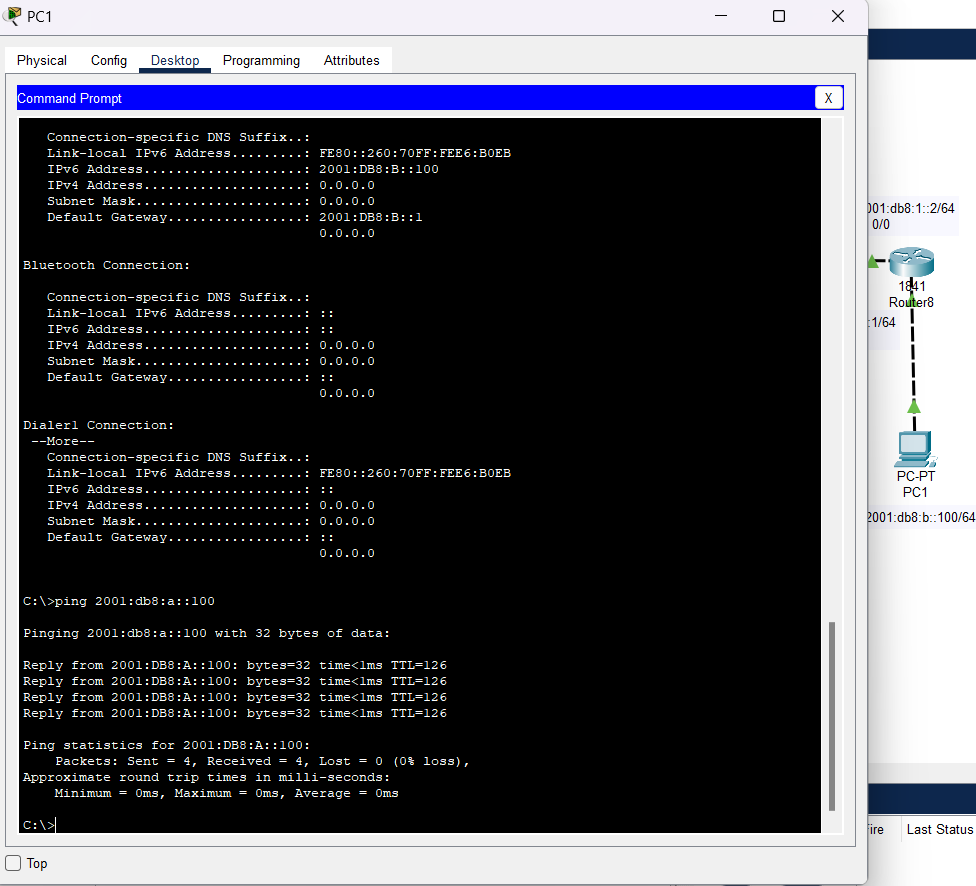
\includegraphics[width=\linewidth]{P2/img/tumod (8).png}
		\caption{Ping PC 2 ke PC 1\label{fig:pingPC2}}
	\end{subfigure}
	\hspace{1cm}
	\caption{Simulasi routing statis}
\end{figure}

Routing dinamis dan hasilnya:
\begin{figure}[H]
	\centering
		\begin{subfigure}[b]{0.4\linewidth}
			\centering
			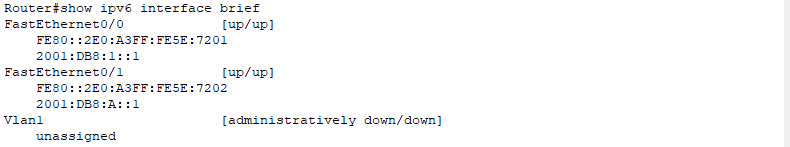
\includegraphics[width=\linewidth]{P2/img/tumod (9).png}
			\caption{Kofigurasi IPv6 router 1\label{fig:konfigurasiR1}}
		\end{subfigure}
		\begin{subfigure}[b]{0.4\linewidth}
			\centering
			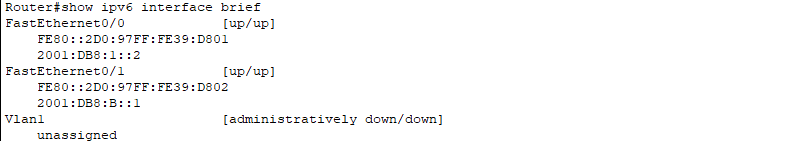
\includegraphics[width=\linewidth]{P2/img/tumod (11).png}
			\caption{Konfigurasi IPv6 router 2\label{fig:konfigurasiR2}}
		\end{subfigure}
		\hspace{1cm}
		\begin{subfigure}[b]{0.4\linewidth}
			\centering
			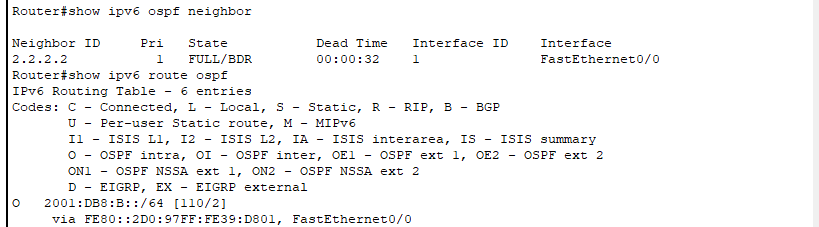
\includegraphics[width=\linewidth]{P2/img/tumod (2).png}
			\caption{Routing OSPFv3 IPv6 router 1\label{fig:routingR1}}
		\end{subfigure}
		\begin{subfigure}[b]{0.4\linewidth}
			\centering
			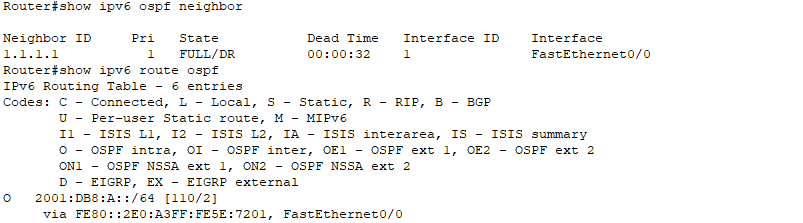
\includegraphics[width=\linewidth]{P2/img/tumod (3).png}
			\caption{Routing OSPFv3 IPv6 router 2\label{fig:routingR2}}
		\end{subfigure}
		\hspace{1cm}
		\begin{subfigure}[b]{0.55\linewidth}
			\centering
			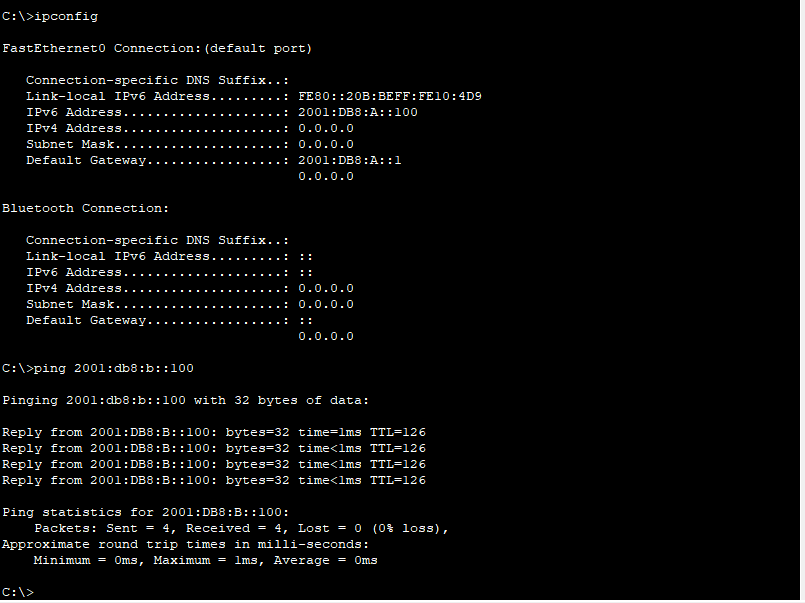
\includegraphics[width=\linewidth]{P2/img/tumod (4).png}
			\caption{Ping PC 1 ke PC 2\label{fig:pingPC1}}
		\end{subfigure}
		\begin{subfigure}[b]{0.5\linewidth}
			\centering
			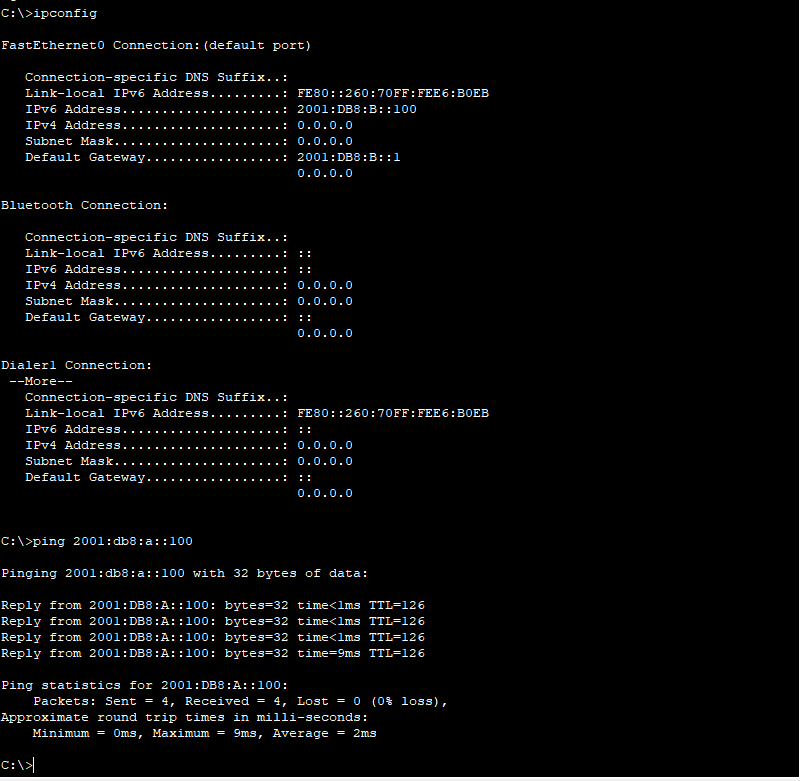
\includegraphics[width=\linewidth]{P2/img/tumod (5).png}
			\caption{Ping PC 2 ke PC 1\label{fig:pingPC2}}
		\end{subfigure}
		\hspace{1cm}
		\caption{Simulasi routing dinamis}
\end{figure}


\section{Kesimpulan}
Berdasarkan hasil yang didapatkan selama praktikum, bisa disimpulkan bahwa untuk membuat/membangun suatu jaringan menggunakan protokol IPv6 dapat menggunakan routing statis dan routing dinamis. Pada percobaan pertama, bisa disimpulkan bahwa antara hasil dan teori sudah sesuai dan dapat dipelajari bahwa konsep dan langkah-langkah untuk melakukan routing statis menggunakan IPv6 sangat mirip dengan routing menggunakan IPv4. Pada percovaab kedua, bisa disimpulkan bahwa antara hasil dan teori sudah sesuai dan dapat dipelajari bahwa untuk melakukan routing dinamis antar router menggunakan IPv6 dapat dilakukan dengan menggunakan protokol OSPFv3.

\section{Lampiran}
\subsection{Dokumentasi saat praktikum}
\begin{figure}[H]
	\centering
	\begin{subfigure}[b]{0.4\linewidth}
		\centering
		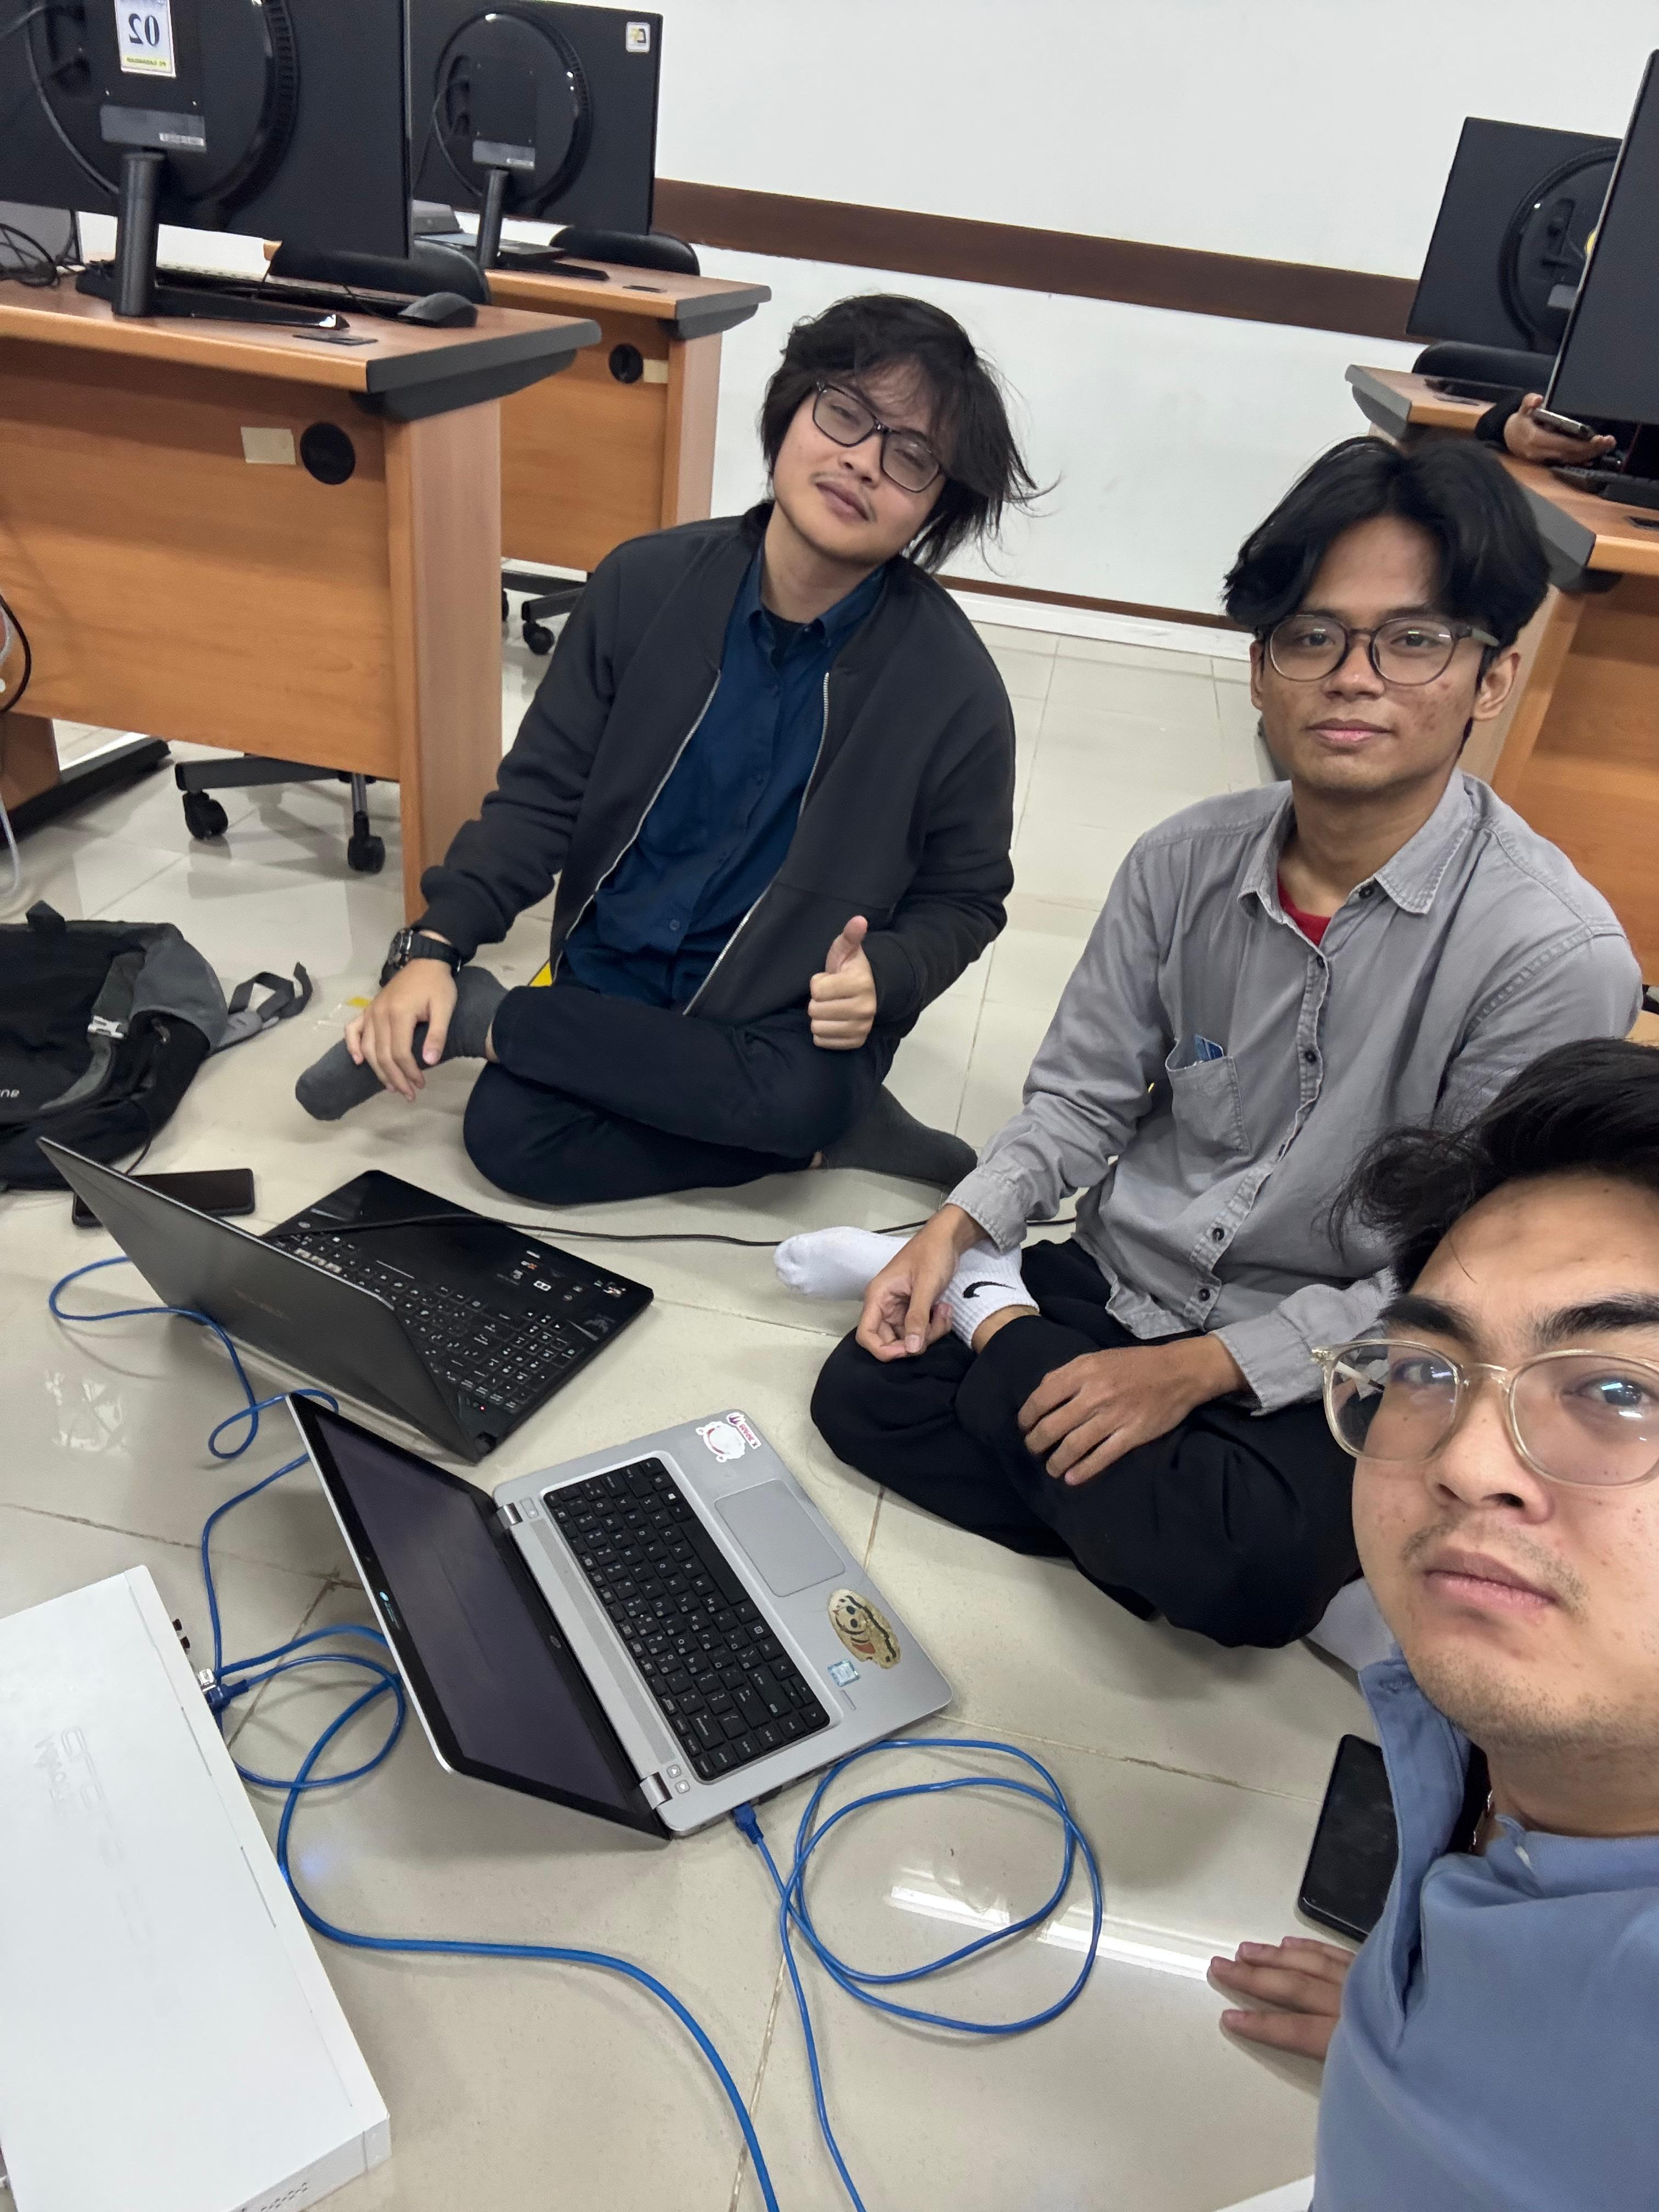
\includegraphics[width=\linewidth]{P2/img/dokum (1).jpg}
	\end{subfigure}
	\begin{subfigure}[b]{0.4\linewidth}
		\centering
		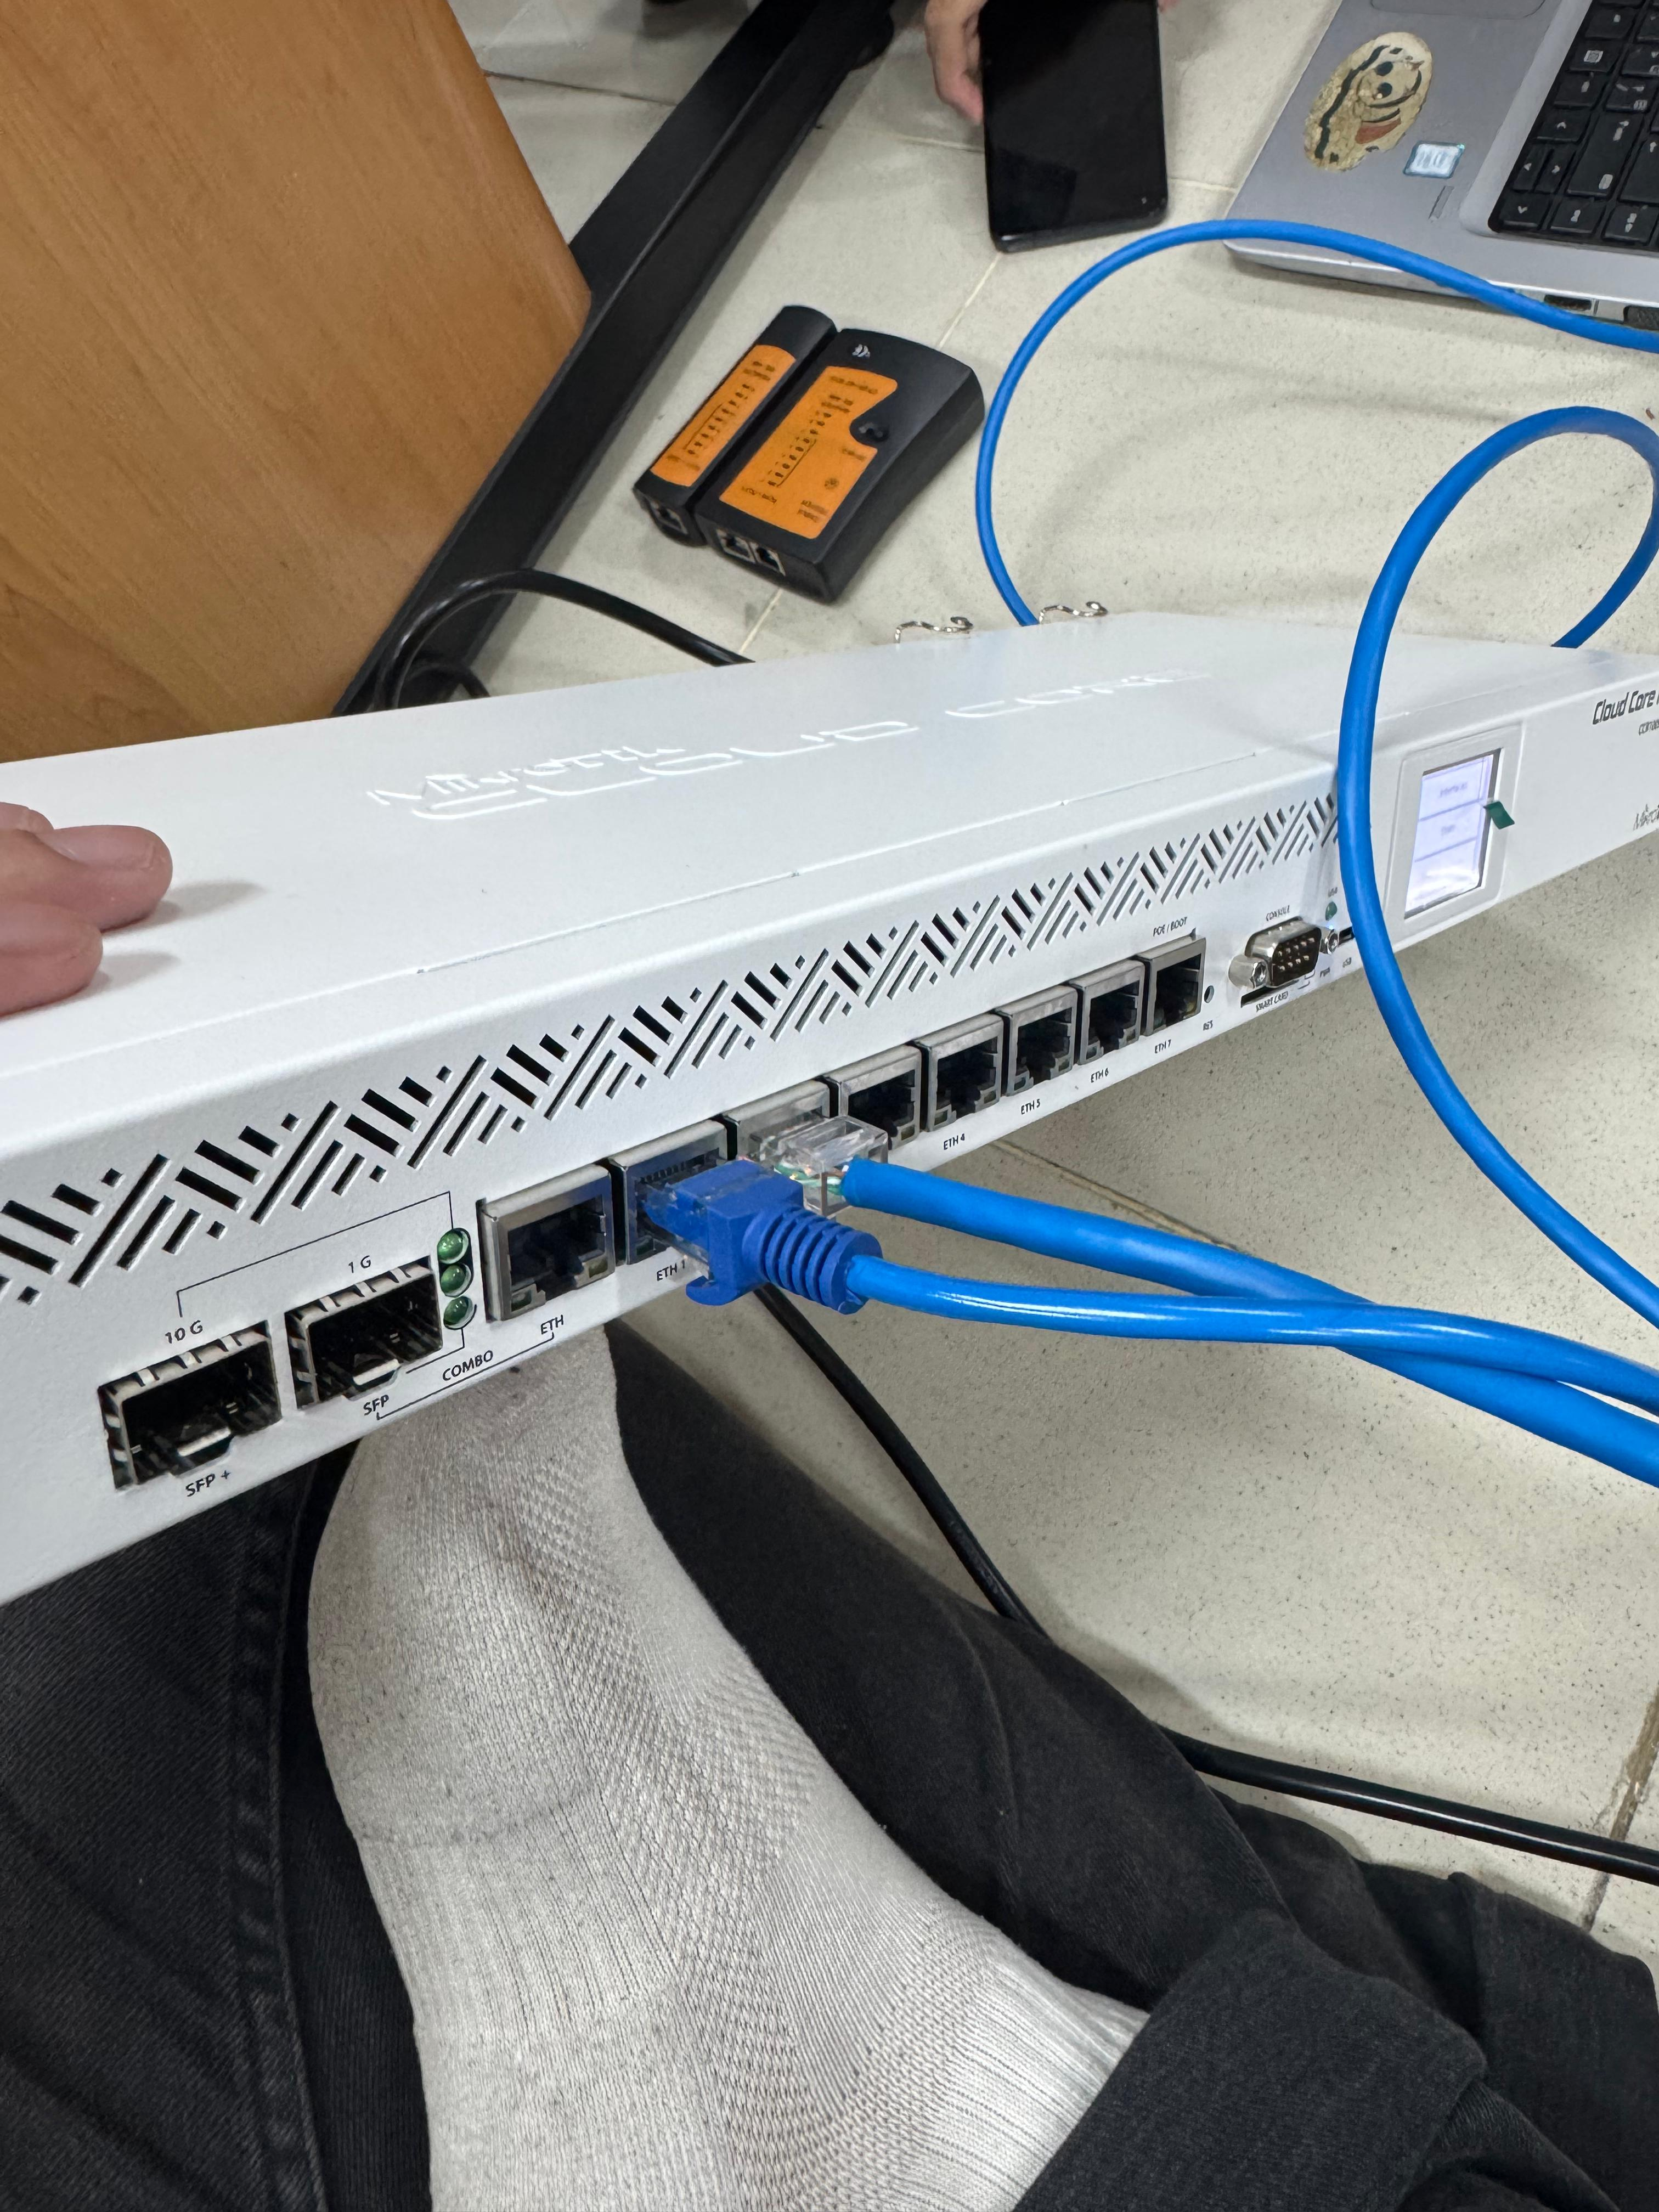
\includegraphics[width=\linewidth]{P2/img/dokum (2).jpg}
	\end{subfigure}
\end{figure}
\begin{figure}[H]
	\centering
	\begin{subfigure}[b]{0.4\linewidth}
		\centering
		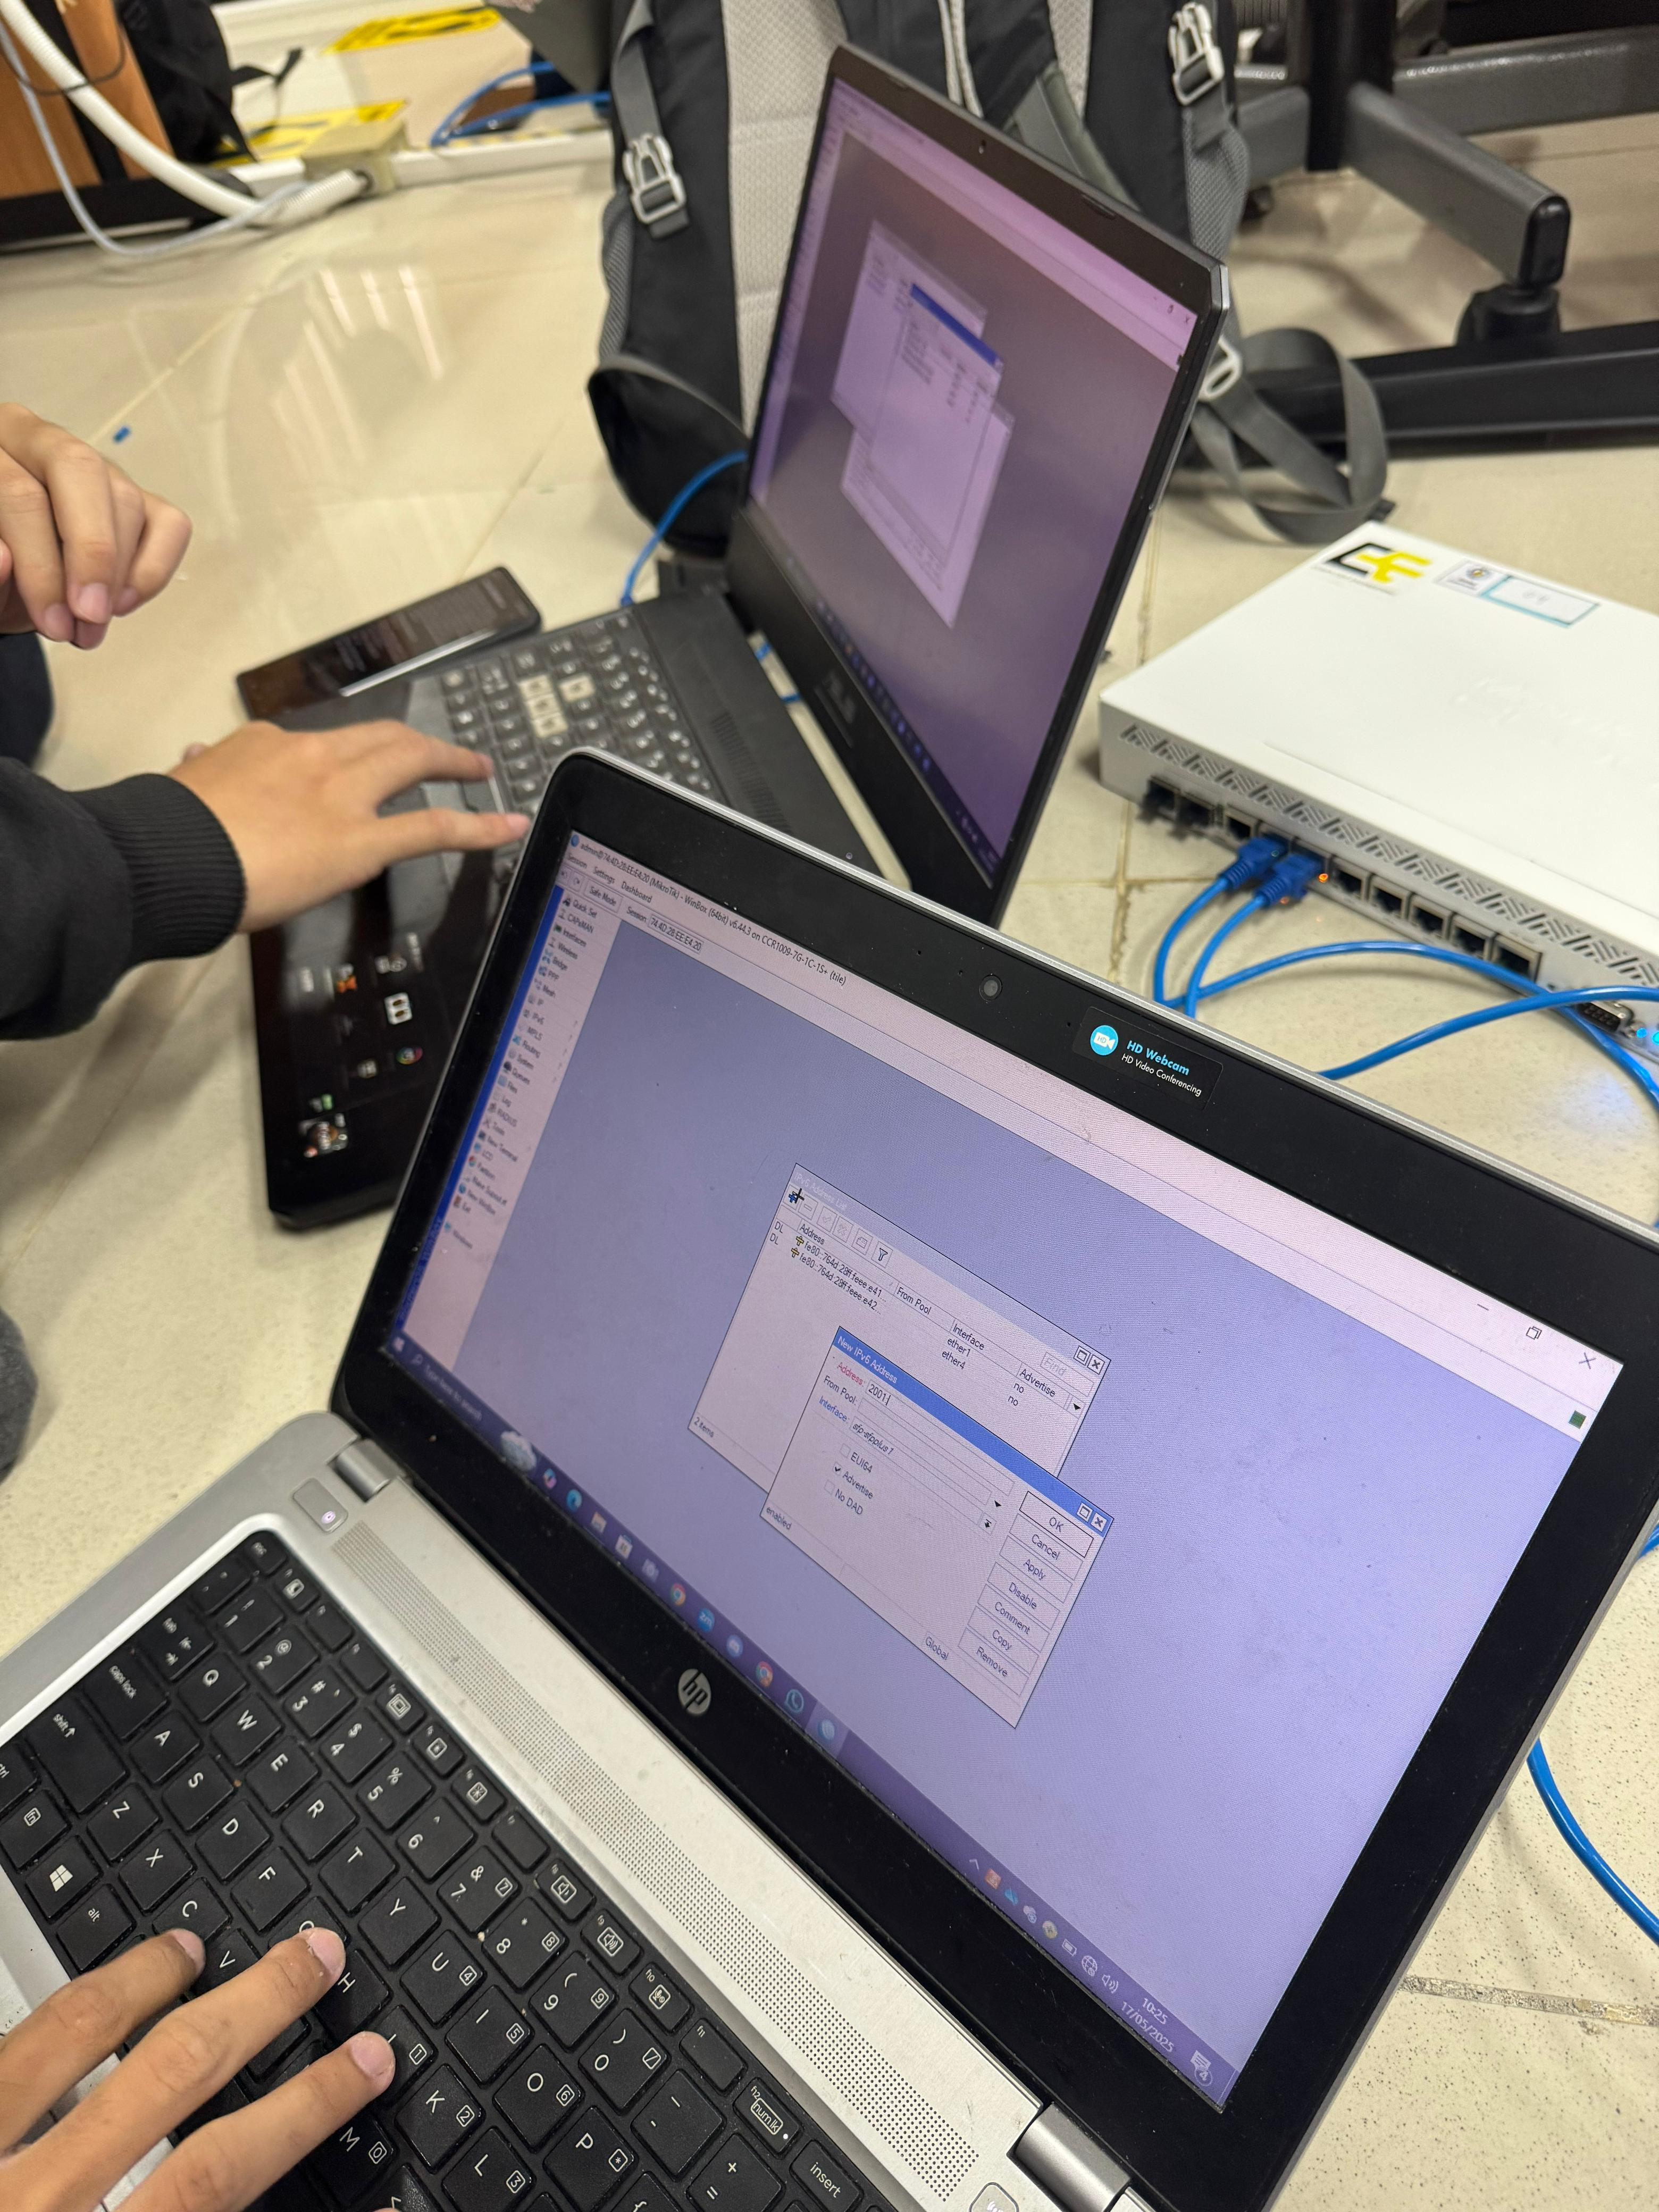
\includegraphics[width=\linewidth]{P2/img/dokum (3).jpg}
	\end{subfigure}
	\begin{subfigure}[b]{0.4\linewidth}
		\centering
		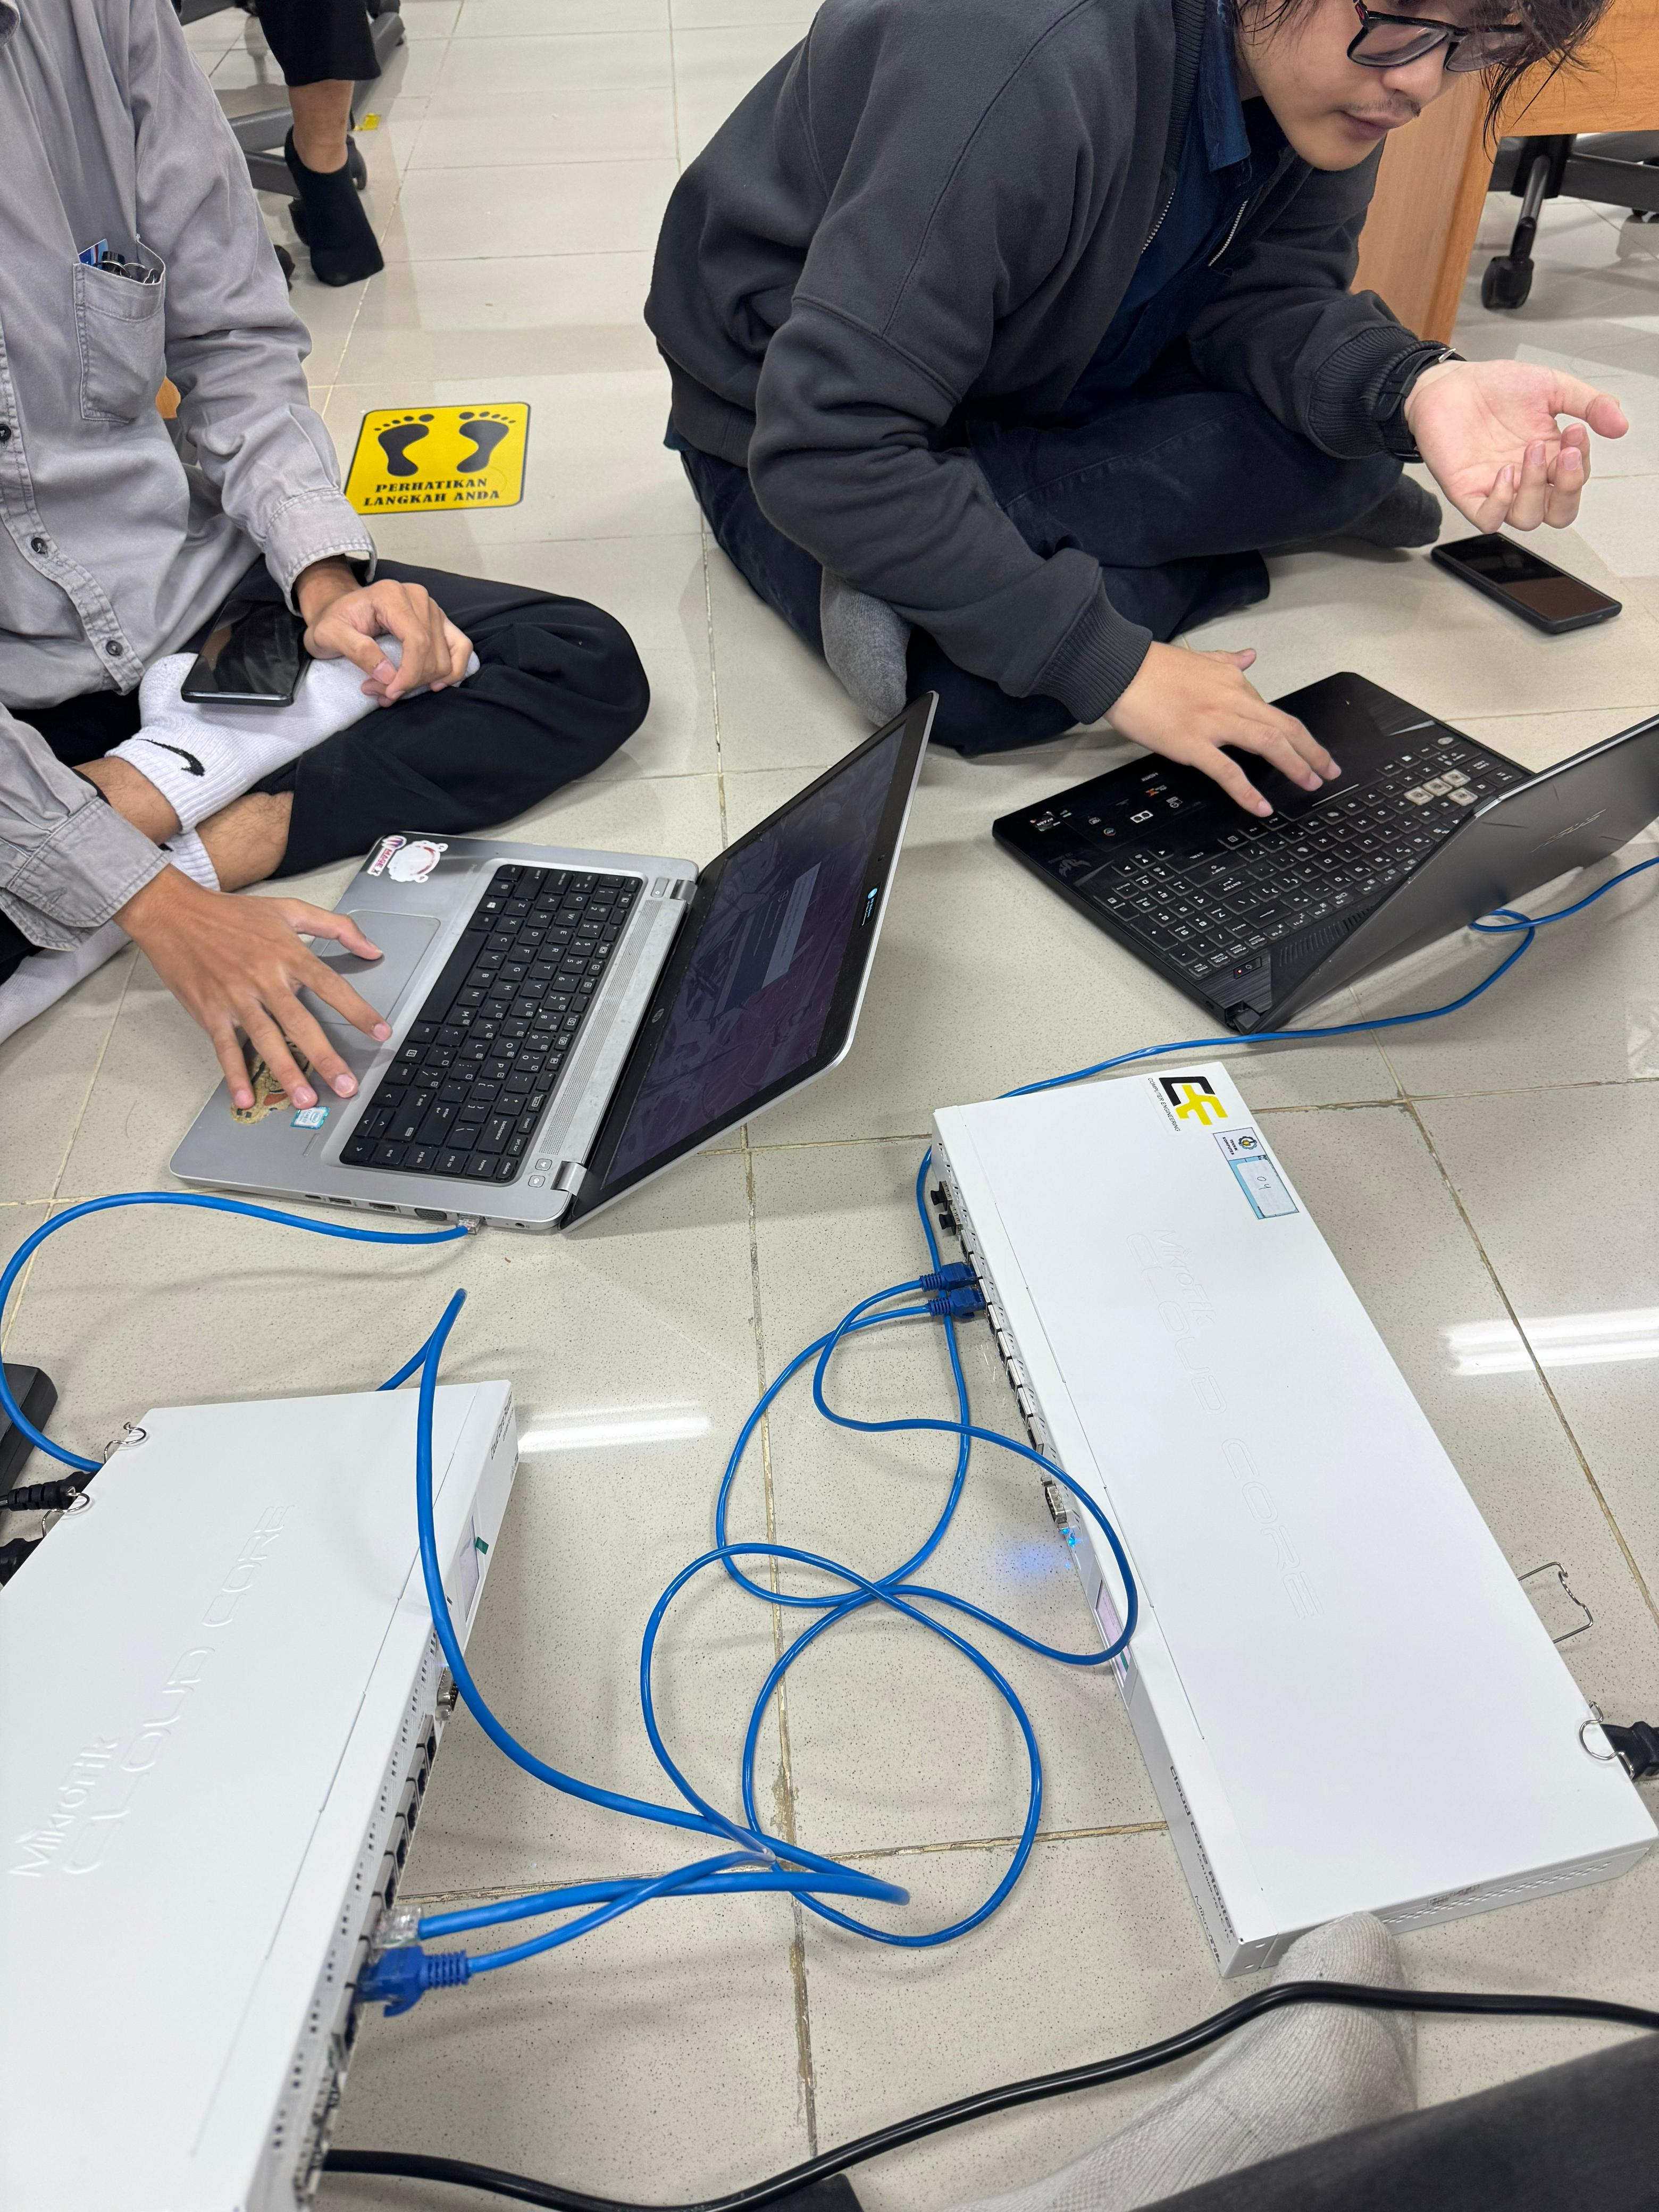
\includegraphics[width=\linewidth]{P2/img/dokum (4).jpg}
	\end{subfigure}
	\centering
\end{figure}
\begin{figure}[H]
	\begin{subfigure}[b]{0.4\linewidth}
		\centering
		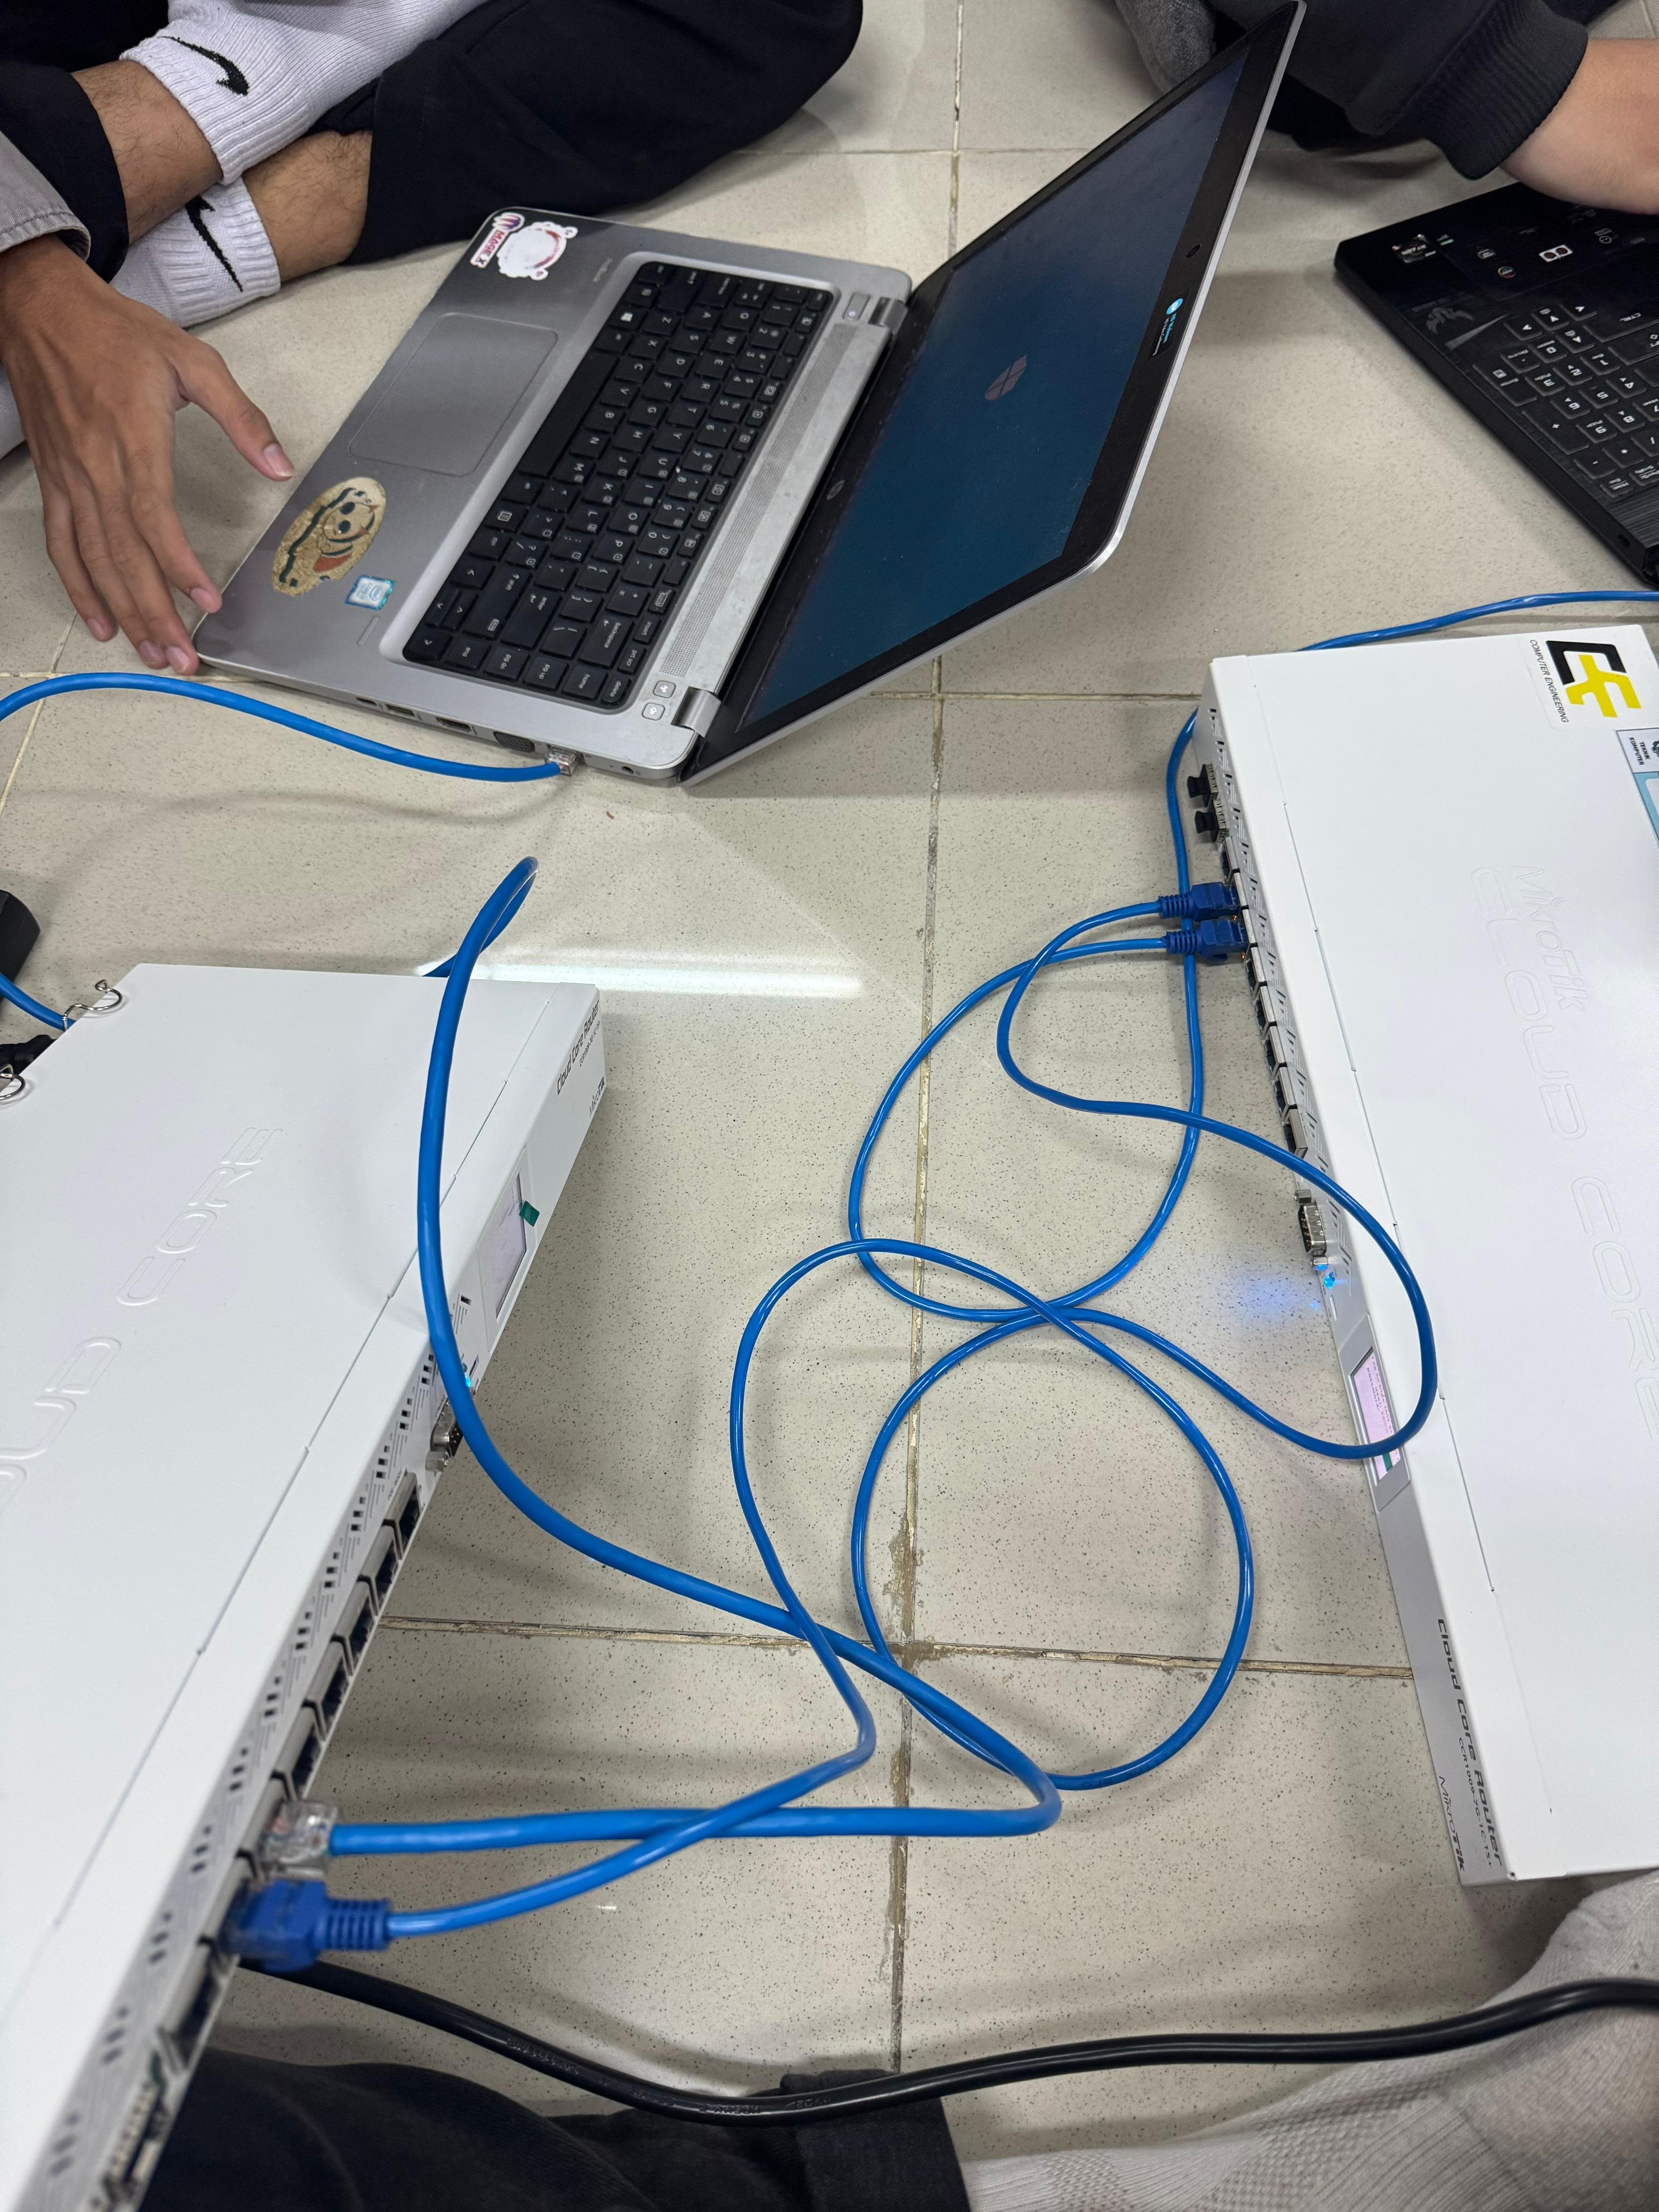
\includegraphics[width=\linewidth]{P2/img/dokum (5).jpg}
	\end{subfigure}
	\begin{subfigure}[b]{0.4\linewidth}
		\centering
		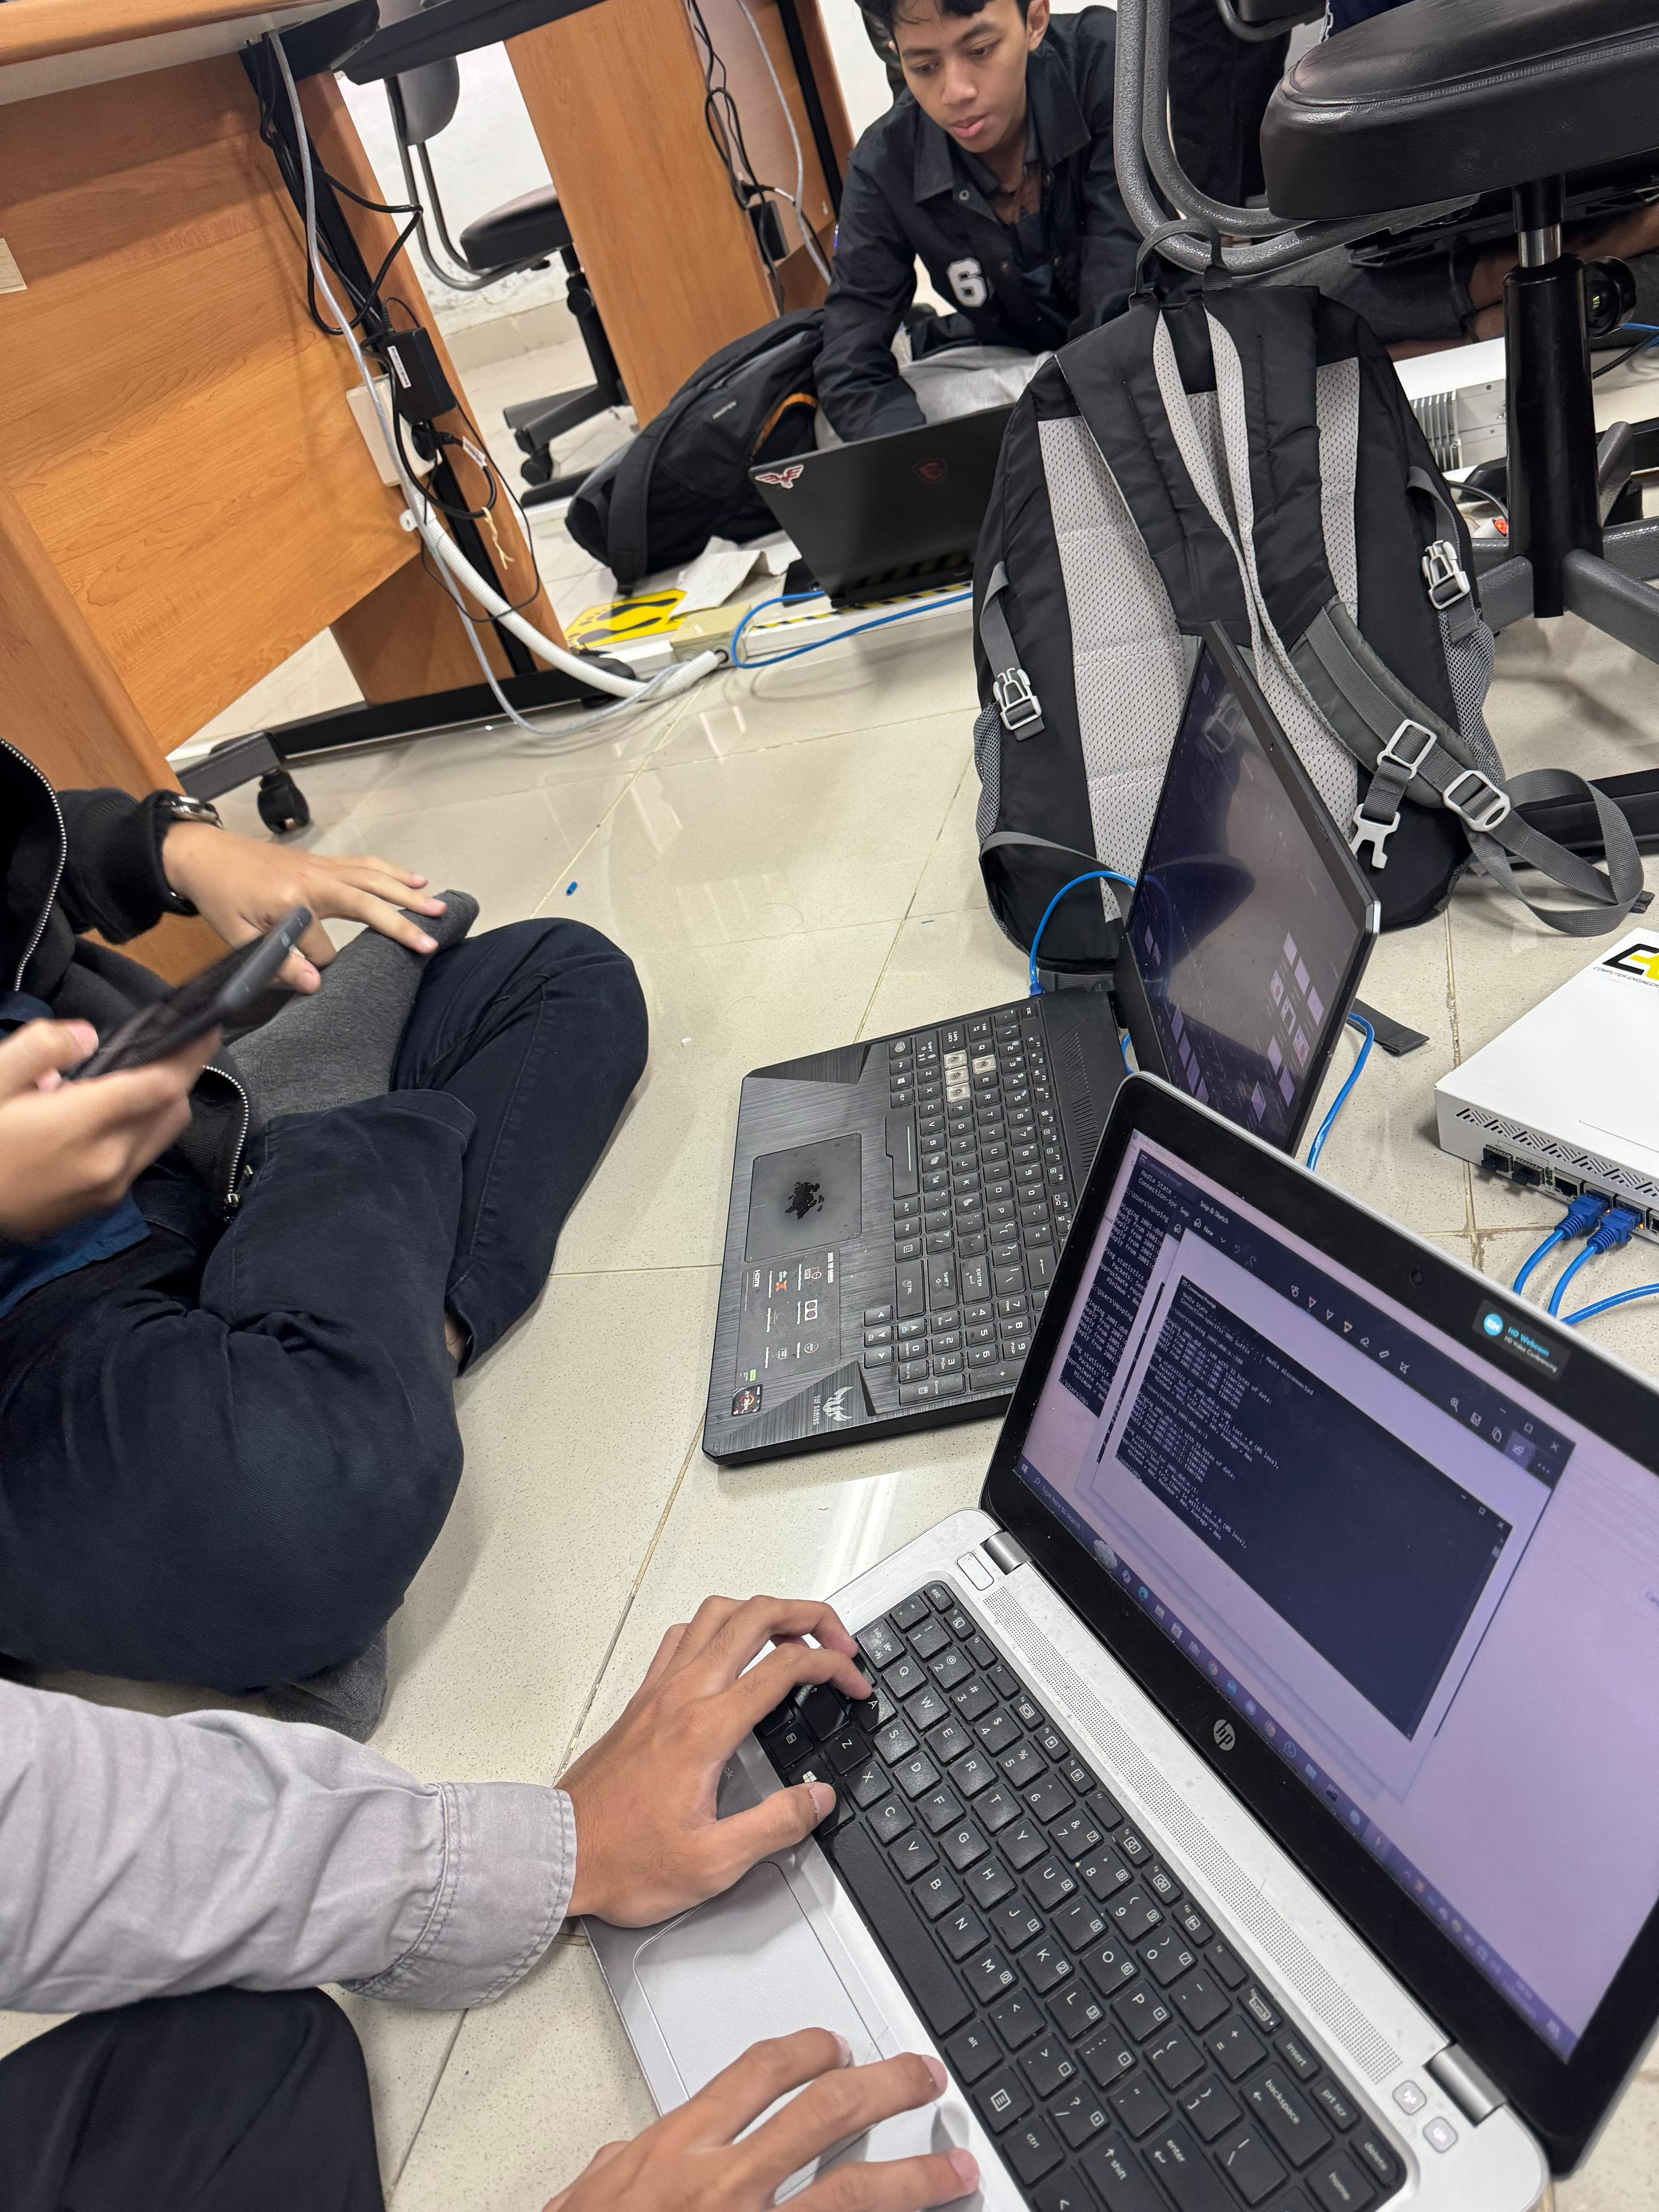
\includegraphics[width=\linewidth]{P2/img/dokum (6).jpg}
	\end{subfigure}
	\begin{subfigure}[b]{0.4\linewidth}
		\centering
		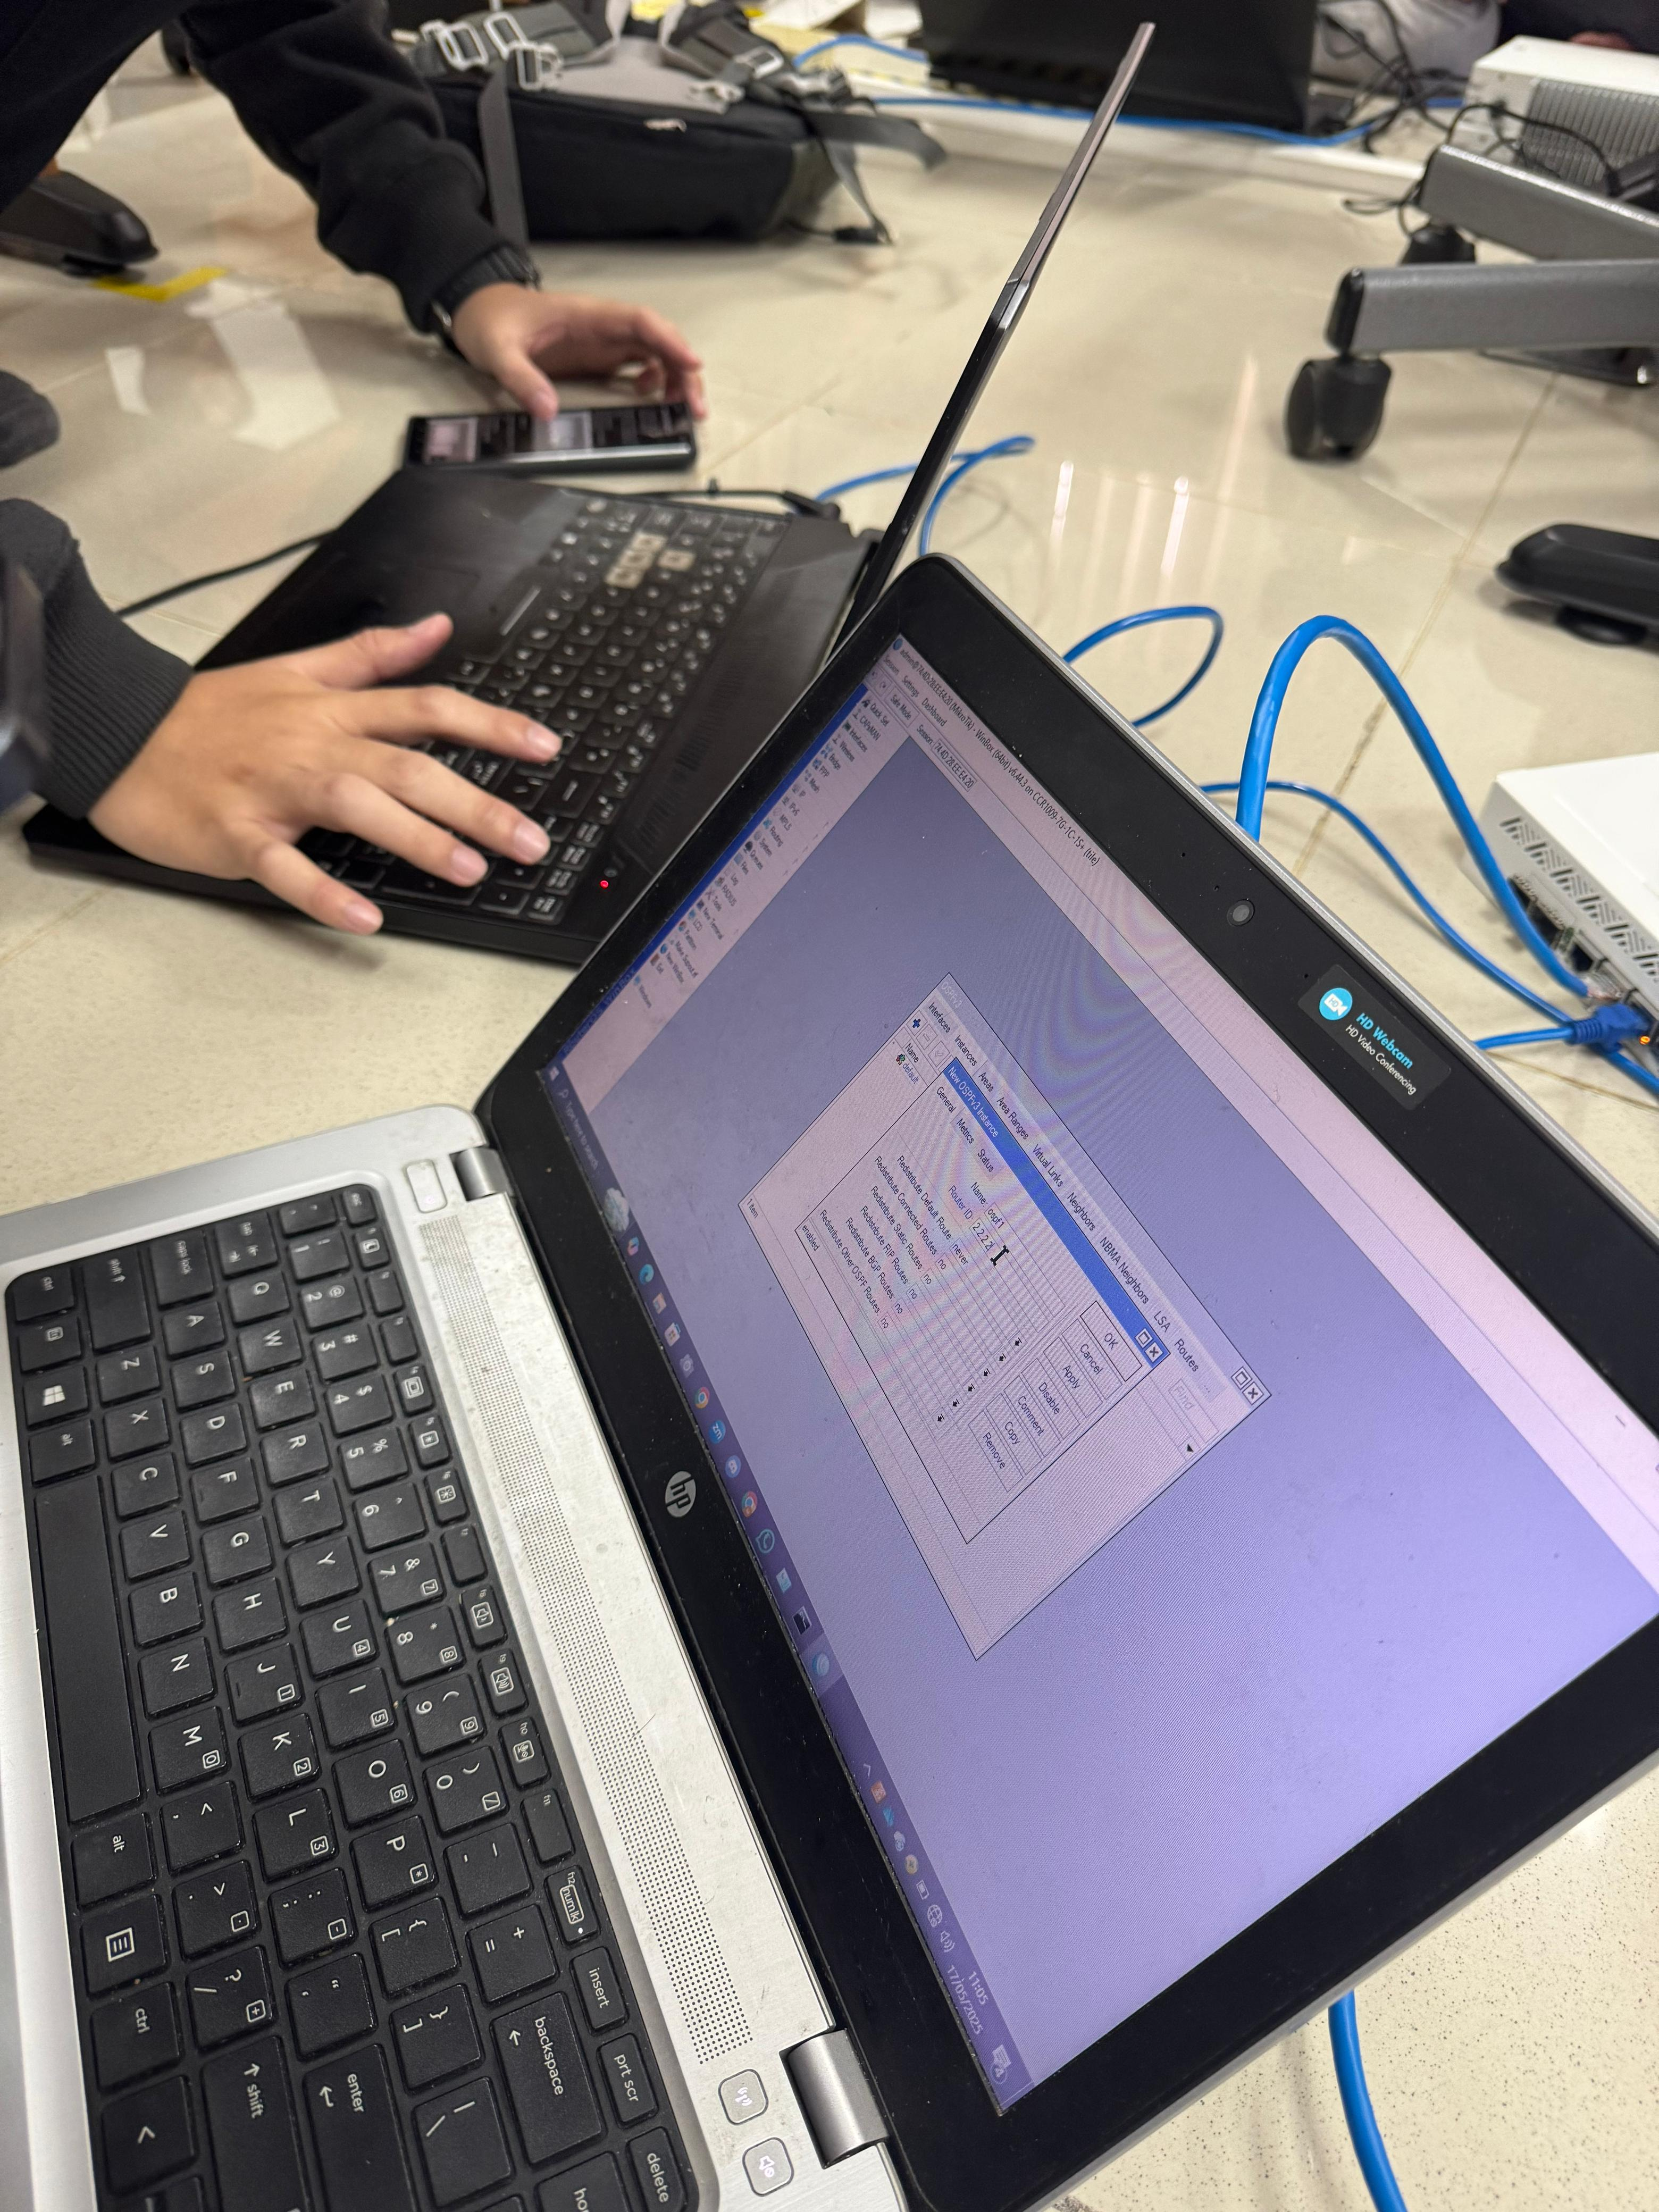
\includegraphics[width=\linewidth]{P2/img/dokum (7).jpg}
	\end{subfigure}
	\caption{Dokumentasi praktikum}
\end{figure}